\chapter{THIẾT KẾ HỆ THỐNG}
Pha thiết kế chuyển kết quả phân tích thành cấu trúc phần mềm có thể hiện thực: kiến trúc, thành phần, giao tiếp, dữ liệu, giao diện và cơ chế đáp ứng yêu cầu phi chức năng. Các lớp phân tích không bị sao chép máy móc thành lớp Python.

\section{Lựa chọn kiến trúc}
\textbf{Modular monolith} phù hợp quy mô nhóm: nhiều module nghiệp vụ trong một backend, giao tiếp qua hàm/\allowbreak{}service có ranh giới; các thao tác kho--mâm--phiên nấu có thể dùng một giao dịch PostgreSQL. Tách thành microservice ngay sẽ phải giải quyết nhất quán phân tán và vận hành nhiều dịch vụ mà chưa có số liệu chứng minh nhu cầu.

Phần xử lý ảnh chạy trong worker độc lập để không giữ request HTTP trong suốt suy luận. API ghi scan, commit rồi đưa job vào RQ. Nếu enqueue sau commit lỗi, sweeper xử lý bản ghi chưa được đưa vào hàng đợi; vì vậy cần phân biệt ``đã nhận yêu cầu'' với ``đã hoàn thành nhận diện''.

Phân tầng: giao diện \ensuremath{\rightarrow} router/\allowbreak{}validation/\allowbreak{}quyền \ensuremath{\rightarrow} service nghiệp vụ \ensuremath{\rightarrow} SQLAlchemy/\allowbreak{}Unit of Work \ensuremath{\rightarrow} PostgreSQL. Mã hiện tại dùng nhiều module hàm Python, không phải mọi thành phần đều là lớp {\small\texttt{Service}} hoặc {\small\texttt{Repository}}. Bản thiết kế không bịa thêm lớp DAO đã cài đặt; SQLAlchemy Session cùng models đang đảm nhiệm truy cập dữ liệu.

\section{Công nghệ và phụ thuộc thành phần}
{\footnotesize\setlength{\tabcolsep}{0pt}
\begin{longtable}{@{}L{5.133cm}@{\hspace{3mm}}L{5.133cm}@{\hspace{3mm}}L{5.133cm}@{}}
\caption{Công nghệ và phụ thuộc thành phần}\\
\toprule
\textbf{Thành phần} & \textbf{Lựa chọn trong repo} & \textbf{Lý do và đánh đổi} \\
\midrule\endfirsthead
\multicolumn{3}{l}{\small\itshape Bảng \thetable{} (tiếp theo)}\\
\toprule
\textbf{Thành phần} & \textbf{Lựa chọn trong repo} & \textbf{Lý do và đánh đổi} \\
\midrule\endhead
\bottomrule\endfoot
Giao diện & Expo /\allowbreak{} React Native /\allowbreak{} TypeScript, Android và web & Chia sẻ phần lớn mã; vẫn cần kiểm khác biệt camera, lưu phiên và layout \\ \addlinespace[3pt]
Backend & FastAPI + Pydantic & Hợp đồng dữ liệu rõ, tích hợp Python ML; cần tránh để tác vụ nặng chặn request \\ \addlinespace[3pt]
Nghiệp vụ và dữ liệu & SQLAlchemy + PostgreSQL & Giao dịch, khóa và ràng buộc mạnh; migration phải theo phiên bản \\ \addlinespace[3pt]
Hàng đợi & Valkey + RQ & Đơn giản cho tác vụ nền; cần retry, sweep và giám sát worker \\ \addlinespace[3pt]
Nhận diện & Mô hình xuất ONNX + ONNX Runtime CPU & Tách huấn luyện khỏi phục vụ; phải kiểm phiên bản, mã băm và ánh xạ lớp \\ \addlinespace[3pt]
Ghép mâm & Thuật toán tổ hợp có ràng buộc và điểm xếp hạng & Bảo toàn điều kiện bắt buộc; giảm không gian ứng viên cần đánh giá ảnh hưởng chất lượng \\ \addlinespace[3pt]
Lịch nấu & OR-\allowbreak{}Tools CP-\allowbreak{}SAT & Biểu diễn thứ tự bước, nguồn lực người/\allowbreak{}bếp; có trạng thái relaxed/\allowbreak{}fallback khi cần \\ \addlinespace[3pt]
Lưu tệp & Ổ đĩa riêng, nginx tải sau kiểm quyền & Dễ vận hành một máy; mở rộng nhiều máy cần shared/\allowbreak{}object storage \\ \addlinespace[3pt]
Triển khai & Docker Compose, nginx, tunnel, CI frontend và pull deployment & Tái lập được bản frontend; máy chủ và sao lưu vẫn là điểm cần giám sát \\ \addlinespace[3pt]
\end{longtable}}
\begin{figure}[H]\centering
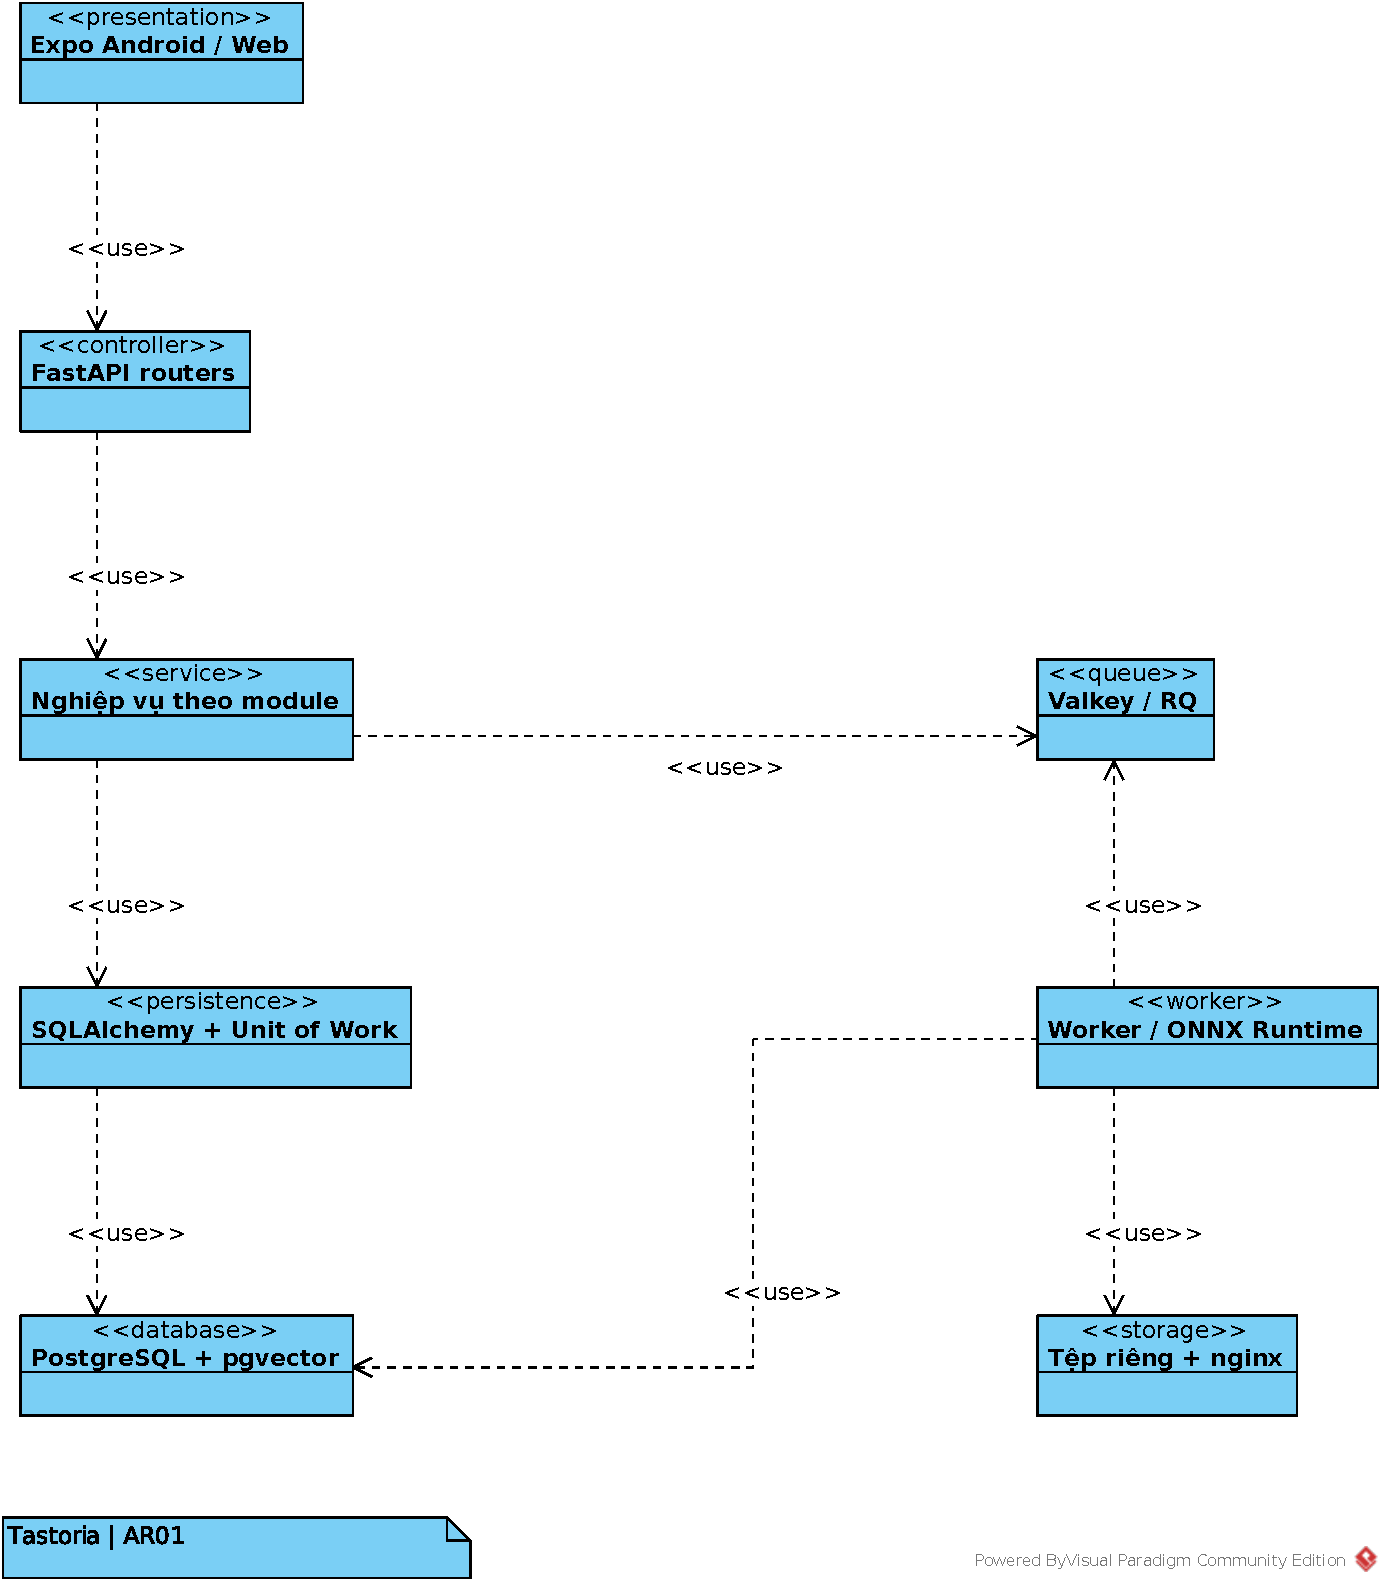
\includegraphics[width=0.96\linewidth,height=0.75\textheight,keepaspectratio]{assets/AR01.pdf}
\caption{AR01 --- Phân tầng và phụ thuộc giữa các khối}\label{fig:Bao-cao-Tastoria:13}
\end{figure}
AR01 dùng UML dependency \guillemotleft{}use\guillemotright{}. Mũi tên worker \ensuremath{\rightarrow} queue thể hiện worker sử dụng hàng đợi, không phải hướng chảy dữ liệu. Đây là góc nhìn trách nhiệm/\allowbreak{}phụ thuộc, không phải sơ đồ mạng. PostgreSQL và tệp là kho lưu lâu dài; Valkey không thay thế cơ sở dữ liệu nghiệp vụ.

\section{Chuyển lớp phân tích sang thiết kế}
{\footnotesize\setlength{\tabcolsep}{0pt}
\begin{longtable}{@{}L{3.775cm}@{\hspace{3mm}}L{3.775cm}@{\hspace{3mm}}L{3.775cm}@{\hspace{3mm}}L{3.775cm}@{}}
\caption{Chuyển lớp phân tích sang thiết kế}\\
\toprule
\textbf{Khái niệm phân tích} & \textbf{Lý do tách} & \textbf{Ánh xạ thiết kế} & \textbf{Dữ liệu} \\
\midrule\endfirsthead
\multicolumn{4}{l}{\small\itshape Bảng \thetable{} (tiếp theo)}\\
\toprule
\textbf{Khái niệm phân tích} & \textbf{Lý do tách} & \textbf{Ánh xạ thiết kế} & \textbf{Dữ liệu} \\
\midrule\endhead
\bottomrule\endfoot
Kết quả quét và lô kho & Dự đoán có thể sửa/\allowbreak{}bỏ; lô là tồn kho đã xác nhận & scan.service.confirm gọi pantry.service.apply\_\allowbreak{}scan & scans, scan\_\allowbreak{}items; pantry\_\allowbreak{}lots, pantry\_\allowbreak{}transactions \\ \addlinespace[3pt]
Công thức và món trong mâm & Công thức dùng lại; món trong mâm có khẩu phần và lịch sử thay & catalog cung cấp công thức; meal.service tạo dòng mâm & recipes, recipe\_\allowbreak{}ingredients; meal\_\allowbreak{}plan\_\allowbreak{}items \\ \addlinespace[3pt]
Mâm và phiên nấu & Đề xuất có thể chưa nấu; phiên có thời điểm và trạng thái riêng & meal.service và cooking.service & meal\_\allowbreak{}plans, cook\_\allowbreak{}sessions \\ \addlinespace[3pt]
Biến động kho và số dư & Cần giữ lịch sử để đảo; số dư là giá trị dẫn xuất & pantry.deduct /\allowbreak{} reverse, truy vấn balance & pantry\_\allowbreak{}transactions, v\_\allowbreak{}pantry\_\allowbreak{}lot\_\allowbreak{}balance \\ \addlinespace[3pt]
Phiên bản và triển khai mô hình & Một phiên bản có thể tồn tại nhưng chưa được chọn phục vụ & module mlops, worker nạp artifact & model\_\allowbreak{}versions, model\_\allowbreak{}deployments \\ \addlinespace[3pt]
\end{longtable}}
Ở pha thiết kế, router nhận yêu cầu, service phối hợp nhiều đối tượng, UnitOfWork quản lý giao dịch và ORM entity biểu diễn trạng thái lưu. Ví dụ complete\_\allowbreak{}session không phải phương thức cập nhật đơn lẻ của {\small\texttt{CookSession}}: nó còn cần kho, mâm, sự kiện và kiểm đồng ý.

\begin{figure}[H]\centering
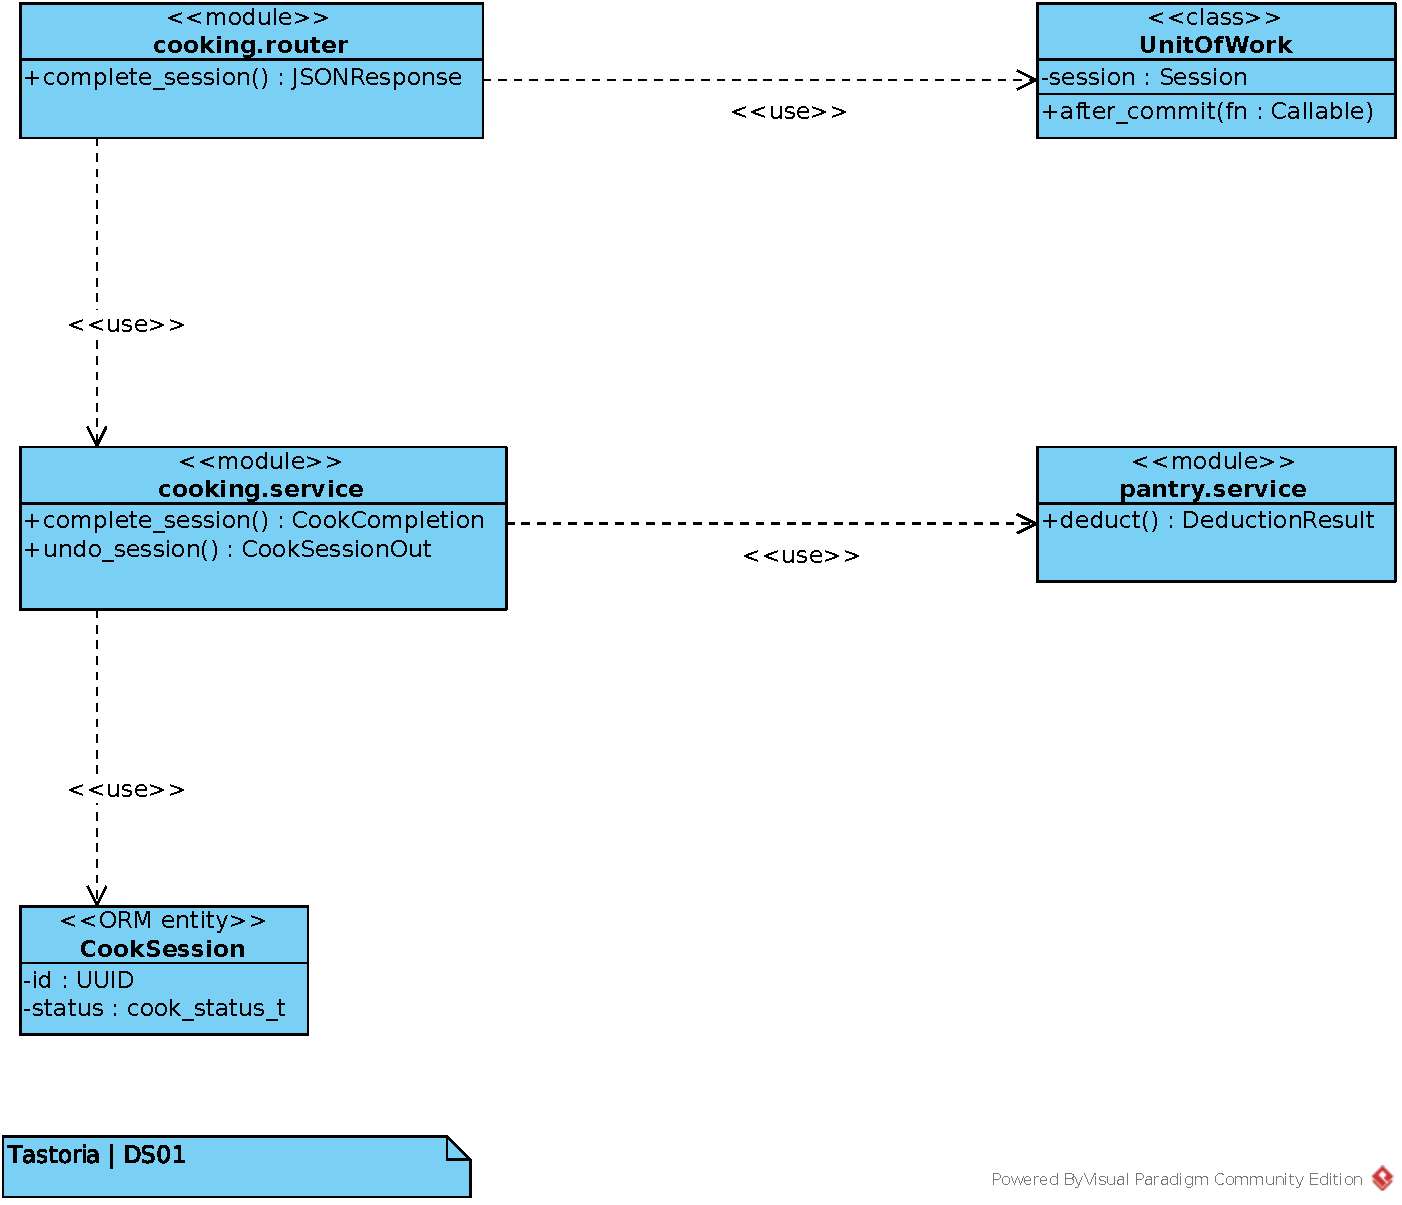
\includegraphics[width=0.96\linewidth,height=0.75\textheight,keepaspectratio]{assets/DS01.pdf}
\caption{DS01 --- Phân bổ trách nhiệm chức năng hoàn tất nấu}\label{fig:Bao-cao-Tastoria:14}
\end{figure}
Tên phương thức trên các sơ đồ thiết kế được rút gọn tham số để dễ đọc; chữ ký thực và việc truyền session/\allowbreak{}dependency cần đối chiếu mã nguồn. \guillemotleft{}module\guillemotright{} biểu diễn module hàm, không khẳng định đó là lớp khởi tạo được.

\section{Thiết kế chi tiết theo chức năng}
Các mục dưới cụ thể hóa trách nhiệm ở mục 3.6 bằng module, giao dịch và tương tác. Hình SQ chỉ biểu diễn các kịch bản được ghi trong chú thích; bảng nhánh và đặc tả UC bổ sung các tình huống khác.

\subsection{Tài khoản, hồ sơ và quyền dữ liệu}
Các module {\small\texttt{identity}}, {\small\texttt{profile}}, {\small\texttt{privacy}} cùng {\small\texttt{core.\allowbreak{}auth}} chịu trách nhiệm xác thực và quyền. API dùng access token và refresh token xoay vòng; app giữ trạng thái phiên theo nền tảng. Dữ liệu hồ sơ đi qua service để tạo điều kiện bữa ăn, thay vì để bộ ghép mâm đọc tùy ý mọi trường sức khỏe.

Khó nhất là phân biệt quyền đăng nhập với quyền xử lý từng mục đích; rút đồng ý phải tác động cả dữ liệu/\allowbreak{}sự kiện liên quan. Điểm tích hợp là người dùng có thể sử dụng chức năng phù hợp mà không bị buộc đồng ý mọi mục đích nghiên cứu/\allowbreak{}cá nhân hóa.

{\footnotesize\setlength{\tabcolsep}{0pt}
\begin{longtable}{@{}L{5.133cm}@{\hspace{3mm}}L{5.133cm}@{\hspace{3mm}}L{5.133cm}@{}}
\caption{Tài khoản, hồ sơ và quyền dữ liệu}\\
\toprule
\textbf{Bước nghiệp vụ} & \textbf{Trách nhiệm và dữ liệu} & \textbf{Trường hợp cần kiểm} \\
\midrule\endfirsthead
\multicolumn{3}{l}{\small\itshape Bảng \thetable{} (tiếp theo)}\\
\toprule
\textbf{Bước nghiệp vụ} & \textbf{Trách nhiệm và dữ liệu} & \textbf{Trường hợp cần kiểm} \\
\midrule\endhead
\bottomrule\endfoot
Mở thiết lập & Lấy phiên bản điều khoản và hồ sơ hiện có & Điều khoản thay phiên bản trong lúc thao tác \\ \addlinespace[3pt]
Chọn đồng ý & Ghi sự kiện theo từng mục đích & Không chọn sẵn thay người dùng \\ \addlinespace[3pt]
Lưu hồ sơ và dị ứng & Kiểm miền giá trị, chủ sở hữu và mã danh mục & Không sửa hồ sơ tài khoản khác \\ \addlinespace[3pt]
Rút đồng ý & Cập nhật quyền xử lý theo mục đích & Đọc lại trạng thái từ máy chủ, không chỉ đổi công tắc local \\ \addlinespace[3pt]
\end{longtable}}
Điểm khó nằm ở tính nhất quán giữa trạng thái đồng ý và tác vụ sử dụng dữ liệu. Sơ đồ phân tích thể hiện trách nhiệm; phần bảo vệ cụ thể phải được kiểm ở API/\allowbreak{}service, không giao toàn bộ cho biểu mẫu.

\subsection{Quét ảnh và quản lý kho theo lô}
{\small\texttt{scan.\allowbreak{}router/\allowbreak{}\allowbreak{}service}} kiểm đầu vào và tạo scan; {\small\texttt{queue/\allowbreak{}\allowbreak{}worker/\allowbreak{}\allowbreak{}detector/\allowbreak{}\allowbreak{}aggregate}} xử lý nền; {\small\texttt{pantry.\allowbreak{}service}} cập nhật lô. Dữ liệu chính gồm {\small\texttt{scans}}, {\small\texttt{scan\_\allowbreak{}\allowbreak{}images}}, {\small\texttt{detections}}, {\small\texttt{scan\_\allowbreak{}\allowbreak{}items}}, {\small\texttt{pantry\_\allowbreak{}\allowbreak{}lots}}, {\small\texttt{pantry\_\allowbreak{}\allowbreak{}transactions}}. Worker không giữ giao dịch DB mở trong toàn bộ suy luận; ghi kết quả có kiểm trạng thái để không hồi sinh một scan đã hết hạn.

Khó nhất là chuyển đầu ra thị giác thành quyết định nhập kho: lớp phát hiện chưa chắc trùng mã nguyên liệu và ảnh không đảm bảo đo đúng lượng. Cách giải là ánh xạ có phiên bản, biểu diễn độ bất định và xác nhận của người dùng. Worker hiện có {\small\texttt{freshness\_\allowbreak{}\allowbreak{}version=None}}; báo cáo không coi mô hình độ tươi là thành phần đã triển khai.

\clearpage\begin{landscape}
\begin{figure}[H]\centering
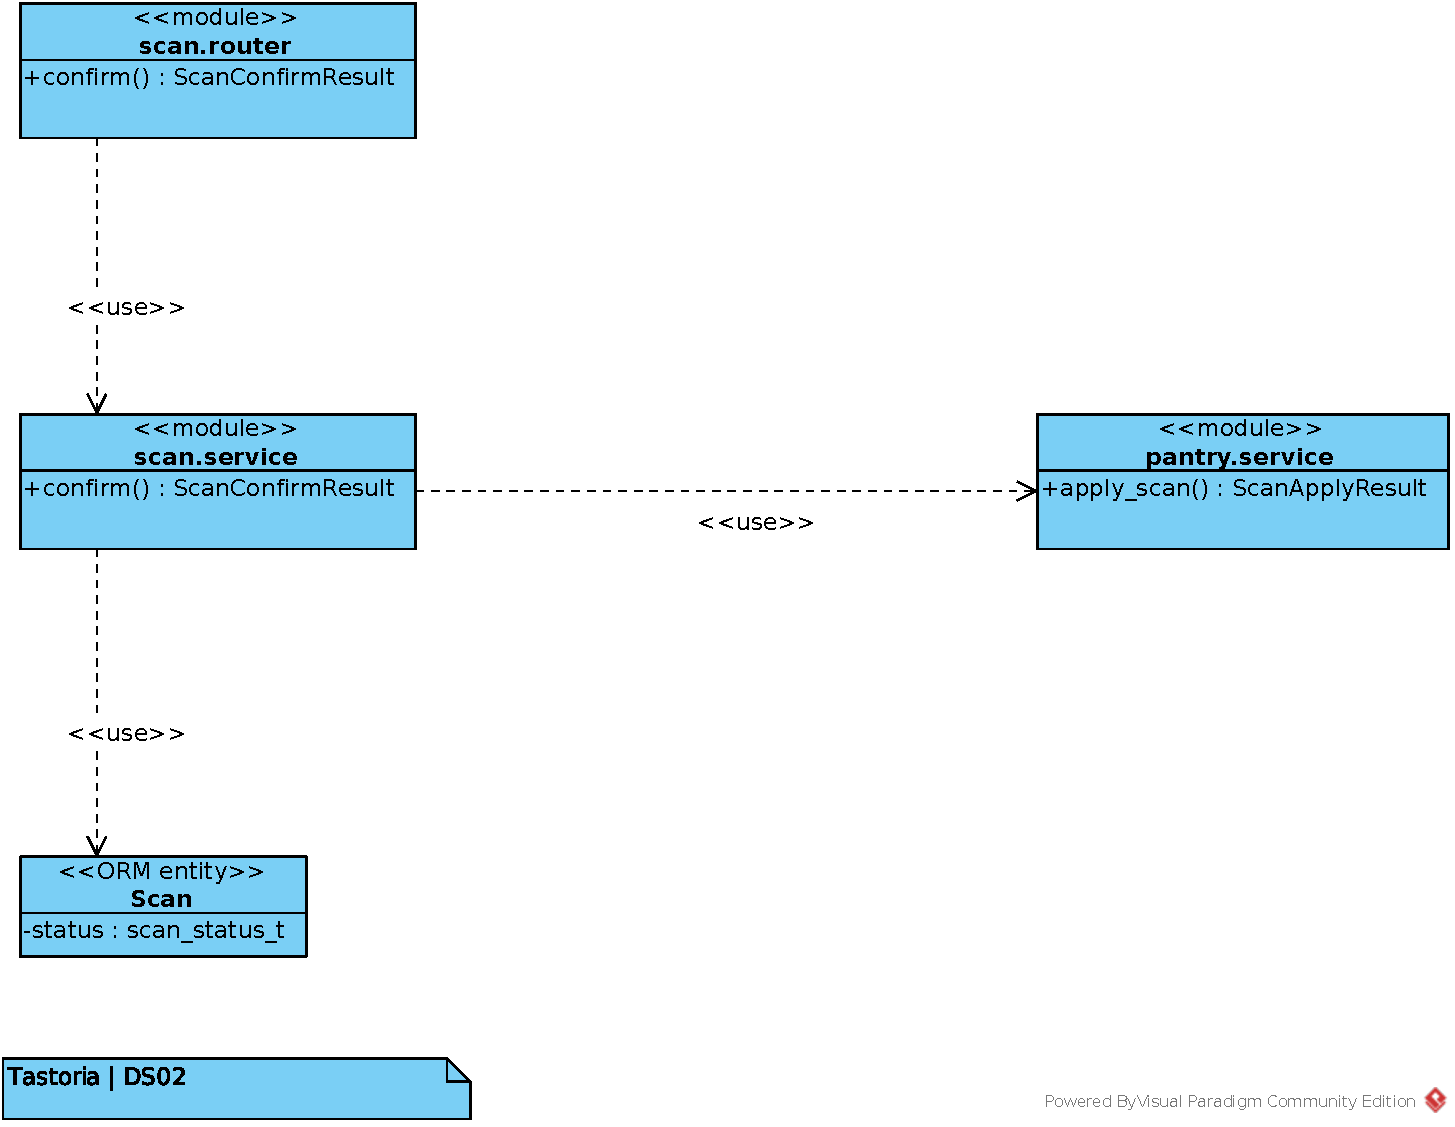
\includegraphics[width=0.96\linewidth,height=0.78\textwidth,keepaspectratio]{assets/DS02.pdf}
\caption{DS02 --- Module thiết kế xác nhận quét}\label{fig:Bao-cao-Tastoria:15}
\end{figure}
\end{landscape}\clearpage
\clearpage\begin{landscape}
\begin{figure}[H]\centering
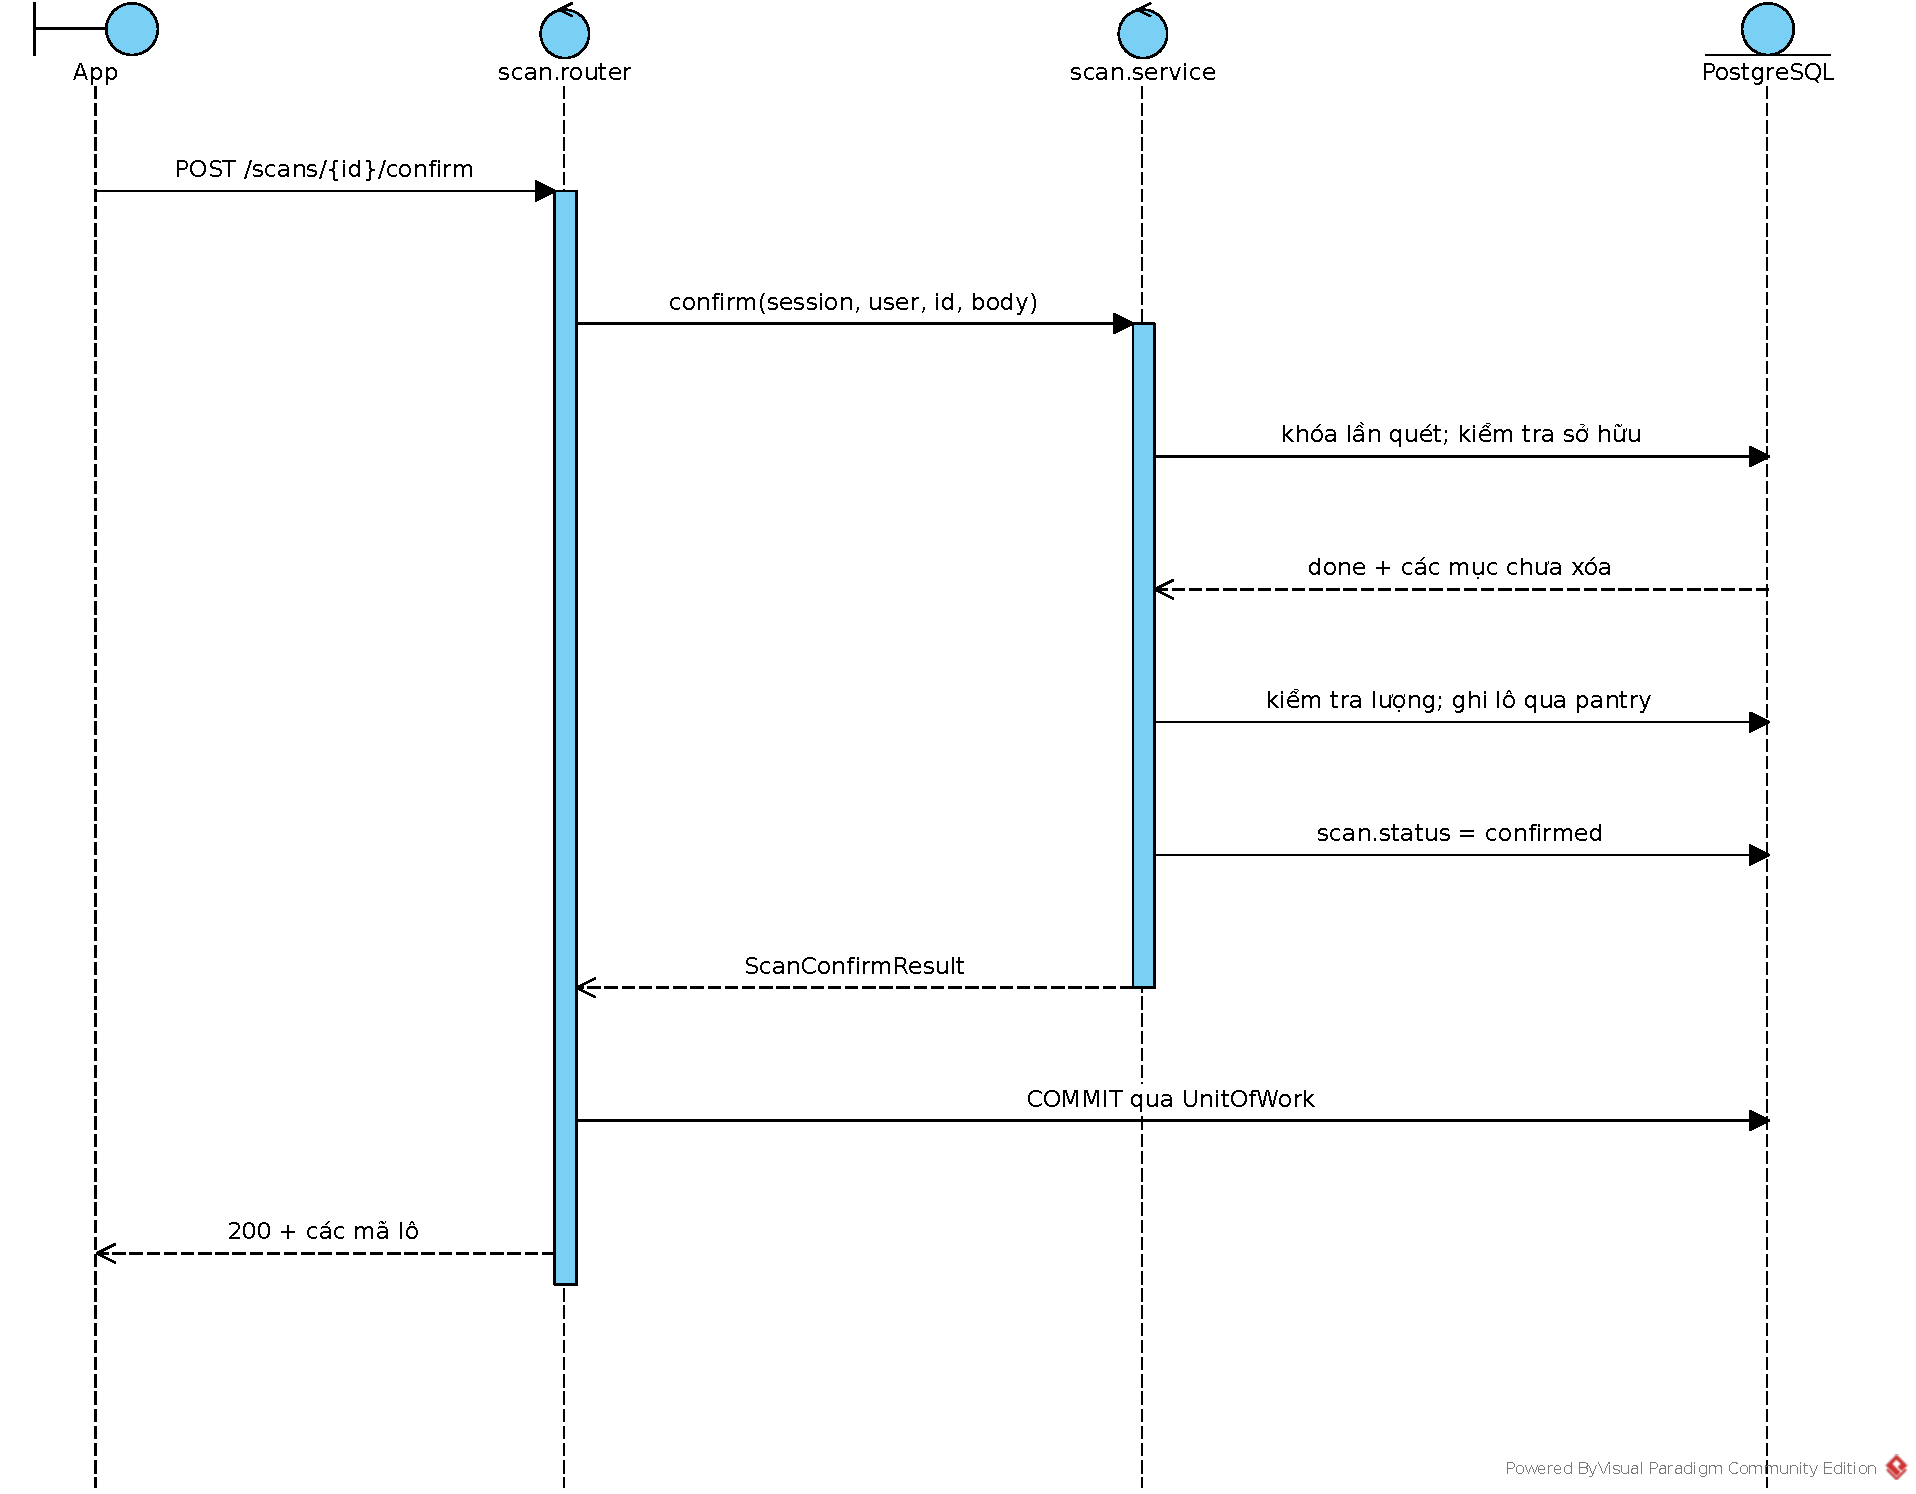
\includegraphics[width=0.96\linewidth,height=0.78\textwidth,keepaspectratio]{assets/SQ03.pdf}
\caption{SQ03 --- Xác nhận lần đầu, với scan đang done}\label{fig:Bao-cao-Tastoria:16}
\end{figure}
\end{landscape}\clearpage
Ở SQ03, scan.service khóa bản ghi scan, kiểm chủ sở hữu, bỏ các mục đã xóa và kiểm lượng. Hàm pantry.apply\_\allowbreak{}scan nhận cùng session, ghi thay đổi kho rồi scan chuyển confirmed. UnitOfWork ở biên request commit trước khi hoàn tất phản hồi. Đường tới PostgreSQL biểu diễn truy vấn/\allowbreak{}ghi qua ORM trong cùng giao dịch, không có nghĩa App được truy cập DB trực tiếp.

{\footnotesize\setlength{\tabcolsep}{0pt}
\begin{longtable}{@{}L{5.133cm}@{\hspace{3mm}}L{5.133cm}@{\hspace{3mm}}L{5.133cm}@{}}
\caption{Quét ảnh và quản lý kho theo lô}\\
\toprule
\textbf{Trường hợp} & \textbf{Xử lý của chức năng} & \textbf{Hậu điều kiện cần kiểm} \\
\midrule\endfirsthead
\multicolumn{3}{l}{\small\itshape Bảng \thetable{} (tiếp theo)}\\
\toprule
\textbf{Trường hợp} & \textbf{Xử lý của chức năng} & \textbf{Hậu điều kiện cần kiểm} \\
\midrule\endhead
\bottomrule\endfoot
scan done, dữ liệu hợp lệ & Áp dụng các mục đã duyệt vào kho & Kho và trạng thái confirmed cùng tồn tại \\ \addlinespace[3pt]
scan confirmed được gửi lại & Trả kết quả đã có qua nhánh replay & Không tạo thêm lô do retry \\ \addlinespace[3pt]
Thiếu mức lượng bắt buộc & Trả lỗi xác thực dữ liệu & Kho giữ nguyên \\ \addlinespace[3pt]
scan chưa done hoặc đã bị bỏ & Từ chối trạng thái không hợp lệ & Không chuyển trạng thái lùi \\ \addlinespace[3pt]
Hai request xác nhận đồng thời & Khóa scan để tuần tự hóa quyết định & Chỉ một lần áp dụng kho \\ \addlinespace[3pt]
\end{longtable}}
SQ03 chỉ vẽ nhánh thành công đầu tiên để giữ hình đọc được; các nhánh trong bảng và đặc tả UC13 là phần của cùng hợp đồng. Độ tin cậy nhận diện phải đánh giá riêng theo dữ liệu ảnh; không suy ra từ việc giao dịch xác nhận chạy đúng.

\subsection{Gợi ý mâm, đổi món và đi chợ}
{\small\texttt{meal.\allowbreak{}service}} điều phối hồ sơ, catalog, kho, bộ xếp hạng, thuật toán {\small\texttt{composer}} và bộ lịch {\small\texttt{schedule}}; {\small\texttt{substitute}} kiểm các cặp thay thế. {\small\texttt{meal\_\allowbreak{}\allowbreak{}plan\_\allowbreak{}\allowbreak{}items}} lưu phiên bản món trong mâm; thay món giữ dấu vết qua dòng bị thay. Năng lượng và lời giải thích lưu theo bối cảnh tạo mâm.

Điểm khó là tiêu chí mềm (gu, sử dụng nguyên liệu sớm, gần mục tiêu năng lượng) không được lấn điều kiện cứng (dị ứng, lượng dùng chung, nguồn lực). Kiểm riêng từng món không đủ; phải kiểm cả tổ hợp. Chưa có kết quả thử người dùng thì không tuyên bố xếp hạng ``phù hợp khẩu vị hơn'' đối thủ.

\begin{figure}[H]\centering
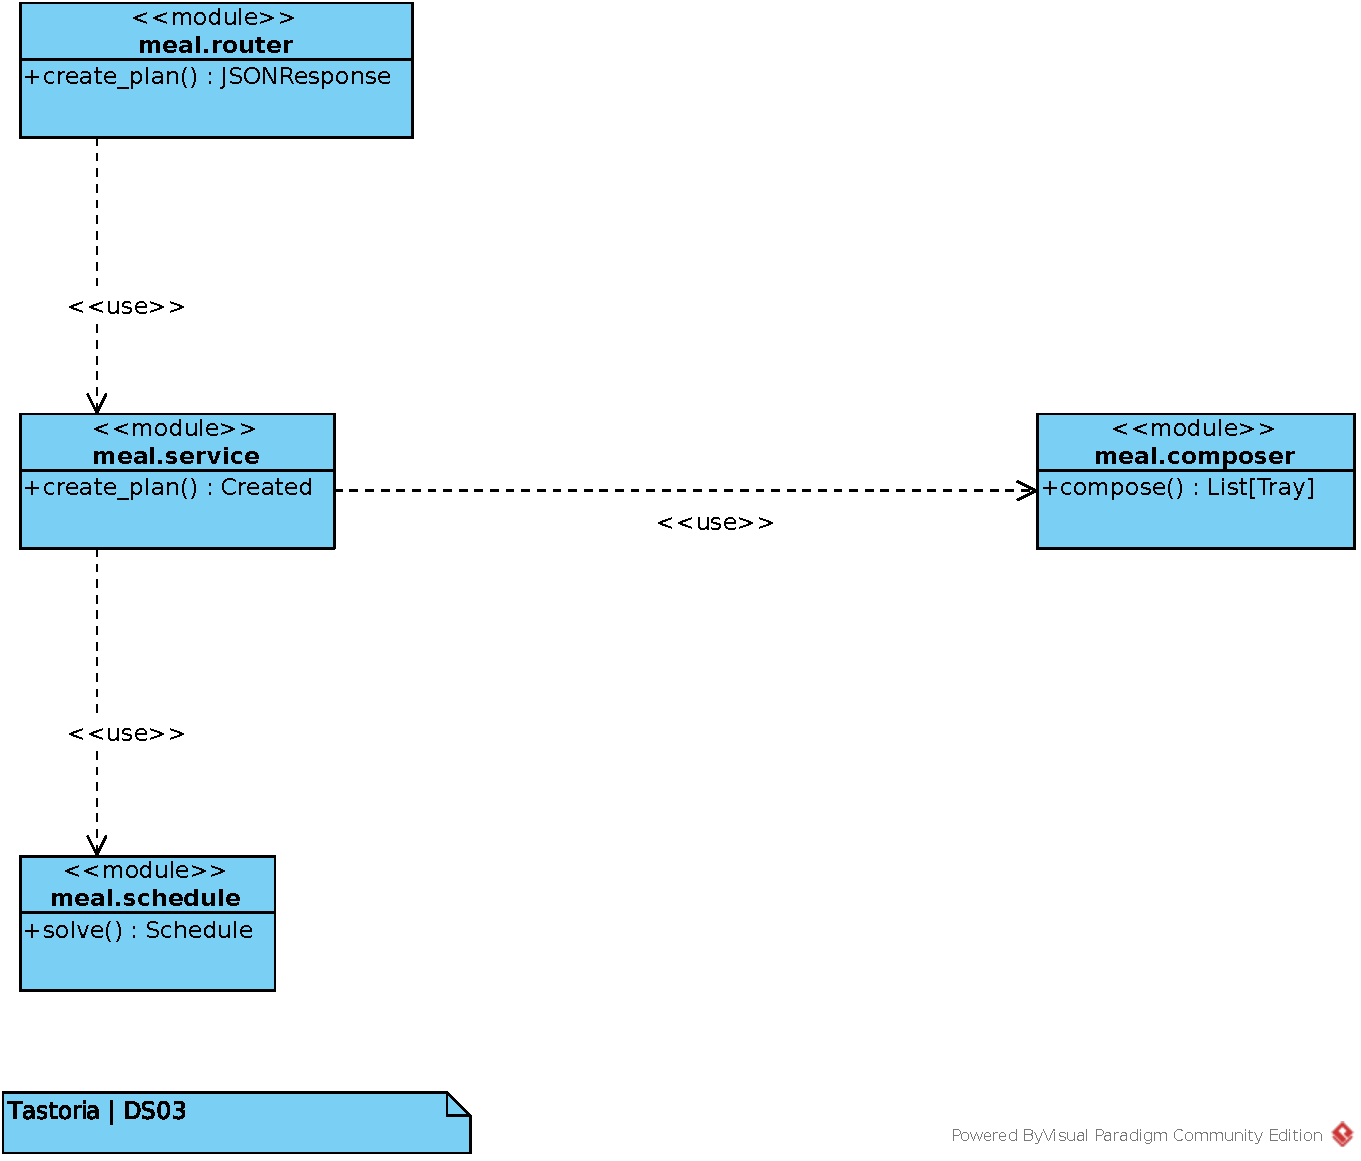
\includegraphics[width=0.96\linewidth,height=0.75\textheight,keepaspectratio]{assets/DS03.pdf}
\caption{DS03 --- Phân bổ điều phối, ghép mâm và lập lịch}\label{fig:Bao-cao-Tastoria:17}
\end{figure}
Trong DS03, meal.router xử lý biên HTTP và khóa yêu cầu; meal.service dựng bối cảnh, lấy ứng viên và điều phối. meal.composer ghép tổ hợp theo cấu trúc mâm; meal.schedule kiểm khả năng sắp lịch. Catalog và truy vấn kho là đầu vào bổ sung, được lược khỏi góc nhìn này và đã thể hiện ở AR01/\allowbreak{}DM01.

Một ví dụ phân tích: kho có 300 g thịt, món mặn cần 200 g và món canh cần 150 g. Hai món riêng lẻ đều không vượt 300 g nhưng tổng 350 g vượt kho. Phải cộng nhu cầu theo mã nguyên liệu sau quy đổi khẩu phần và thay thế, rồi kiểm cả mâm. Các số trên chỉ minh họa bất biến, không phải dữ liệu kiểm thử đã chạy.

{\footnotesize\setlength{\tabcolsep}{0pt}
\begin{longtable}{@{}L{5.133cm}@{\hspace{3mm}}L{5.133cm}@{\hspace{3mm}}L{5.133cm}@{}}
\caption{Gợi ý mâm, đổi món và đi chợ}\\
\toprule
\textbf{Tình huống} & \textbf{Quyết định} & \textbf{Tác động dữ liệu} \\
\midrule\endfirsthead
\multicolumn{3}{l}{\small\itshape Bảng \thetable{} (tiếp theo)}\\
\toprule
\textbf{Tình huống} & \textbf{Quyết định} & \textbf{Tác động dữ liệu} \\
\midrule\endhead
\bottomrule\endfoot
Có mâm hợp lệ & Xếp hạng, lưu món và lời giải thích & Tạo đề xuất; chưa trừ kho \\ \addlinespace[3pt]
Không đủ lượng dùng chung & Tìm tổ hợp khác hoặc báo không khả thi & Không âm thầm chấp nhận thiếu kho như mâm đủ \\ \addlinespace[3pt]
Người dùng đổi một món & Cố định phần còn lại, kiểm lại toàn mâm & Giữ dấu vết dòng bị thay \\ \addlinespace[3pt]
Thay nguyên liệu & Kiểm cặp thay, dị ứng, tỷ lệ và nhu cầu chung & Lưu lựa chọn thay thế gắn với món \\ \addlinespace[3pt]
Hết thời gian giải lịch & Dùng chế độ dự phòng có ghi trạng thái & Không báo lịch tối ưu khi chỉ có nghiệm dự phòng \\ \addlinespace[3pt]
\end{longtable}}
Khó khăn thuật toán là số tổ hợp tăng nhanh khi thêm món; thu hẹp ứng viên giảm chi phí nhưng có thể bỏ nghiệm tốt. Vì vậy cần đo cả thời gian và tỷ lệ tìm được phương án, lưu cấu hình ứng viên, giới hạn thời gian và bộ dữ liệu khi so sánh.

\subsection{Lịch nấu, hoàn tất, hoàn tác và nhật ký}
{\small\texttt{meal.\allowbreak{}schedule}} dùng CP-\allowbreak{}SAT: NoOverlap cho thao tác chủ động, Cumulative cho bếp, ràng buộc thứ tự bước. {\small\texttt{cooking.\allowbreak{}service}} phối hợp kho và mâm; router dùng idempotency; {\small\texttt{core.\allowbreak{}db.\allowbreak{}UnitOfWork}} commit trước khi trả phản hồi. Đây là hiện thực bằng module hàm, không phải một lớp controller tự giữ mọi nghiệp vụ.

\clearpage\begin{landscape}
\begin{figure}[H]\centering
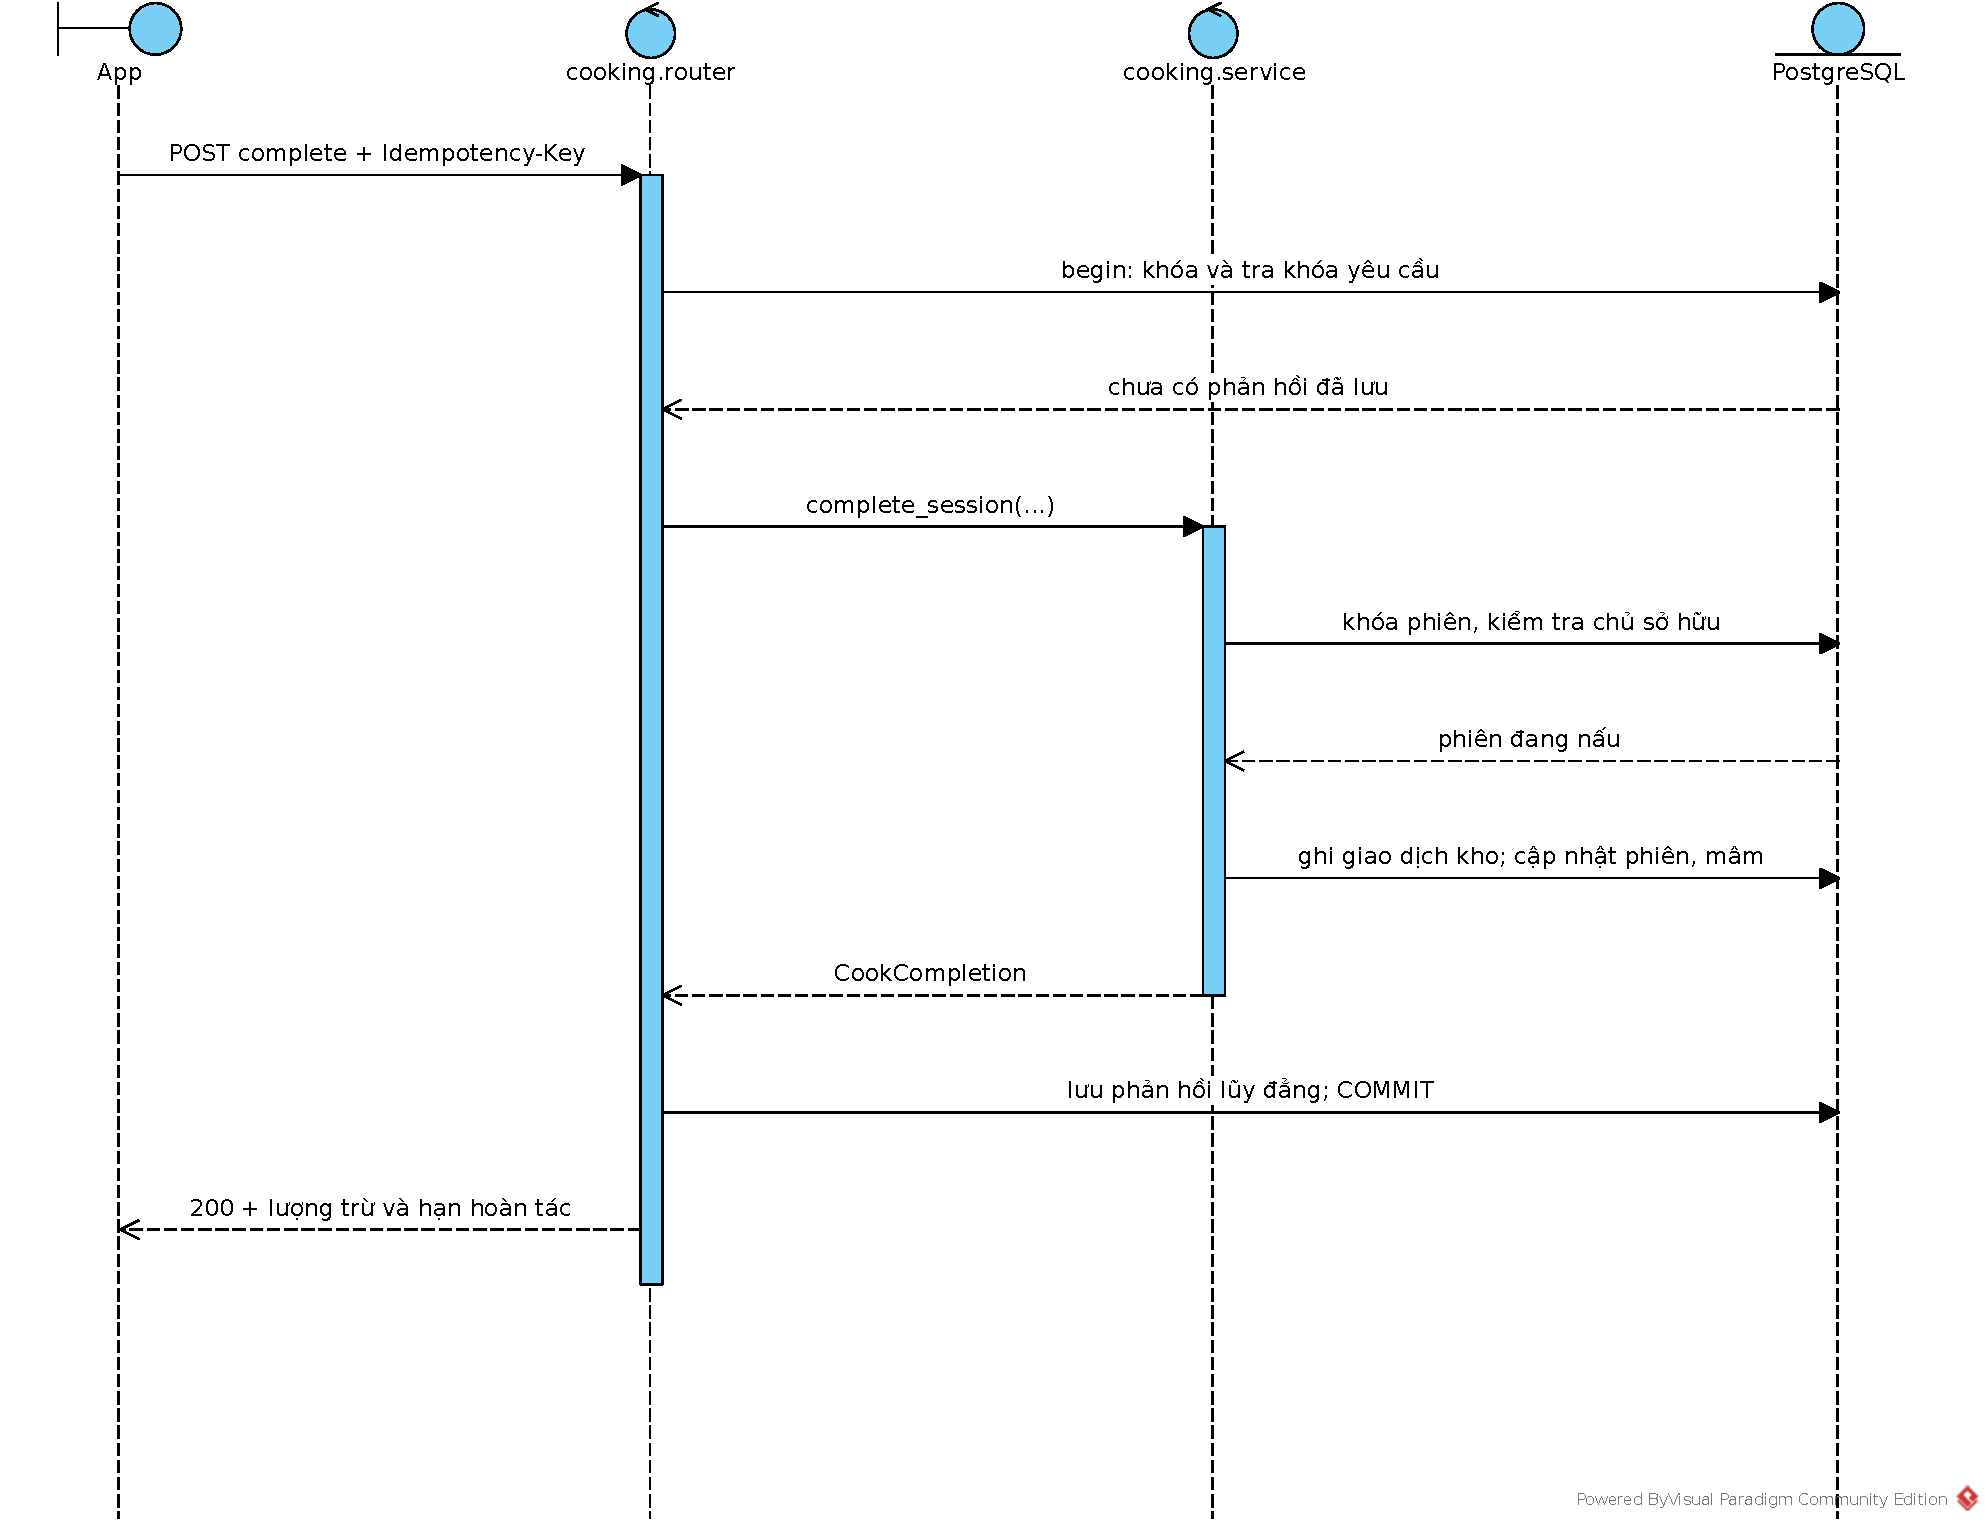
\includegraphics[width=0.96\linewidth,height=0.78\textwidth,keepaspectratio]{assets/SQ01.pdf}
\caption{SQ01 --- Nhánh lần đầu hoàn tất, phiên đang nấu; nhánh replay và lỗi được đặc tả ở UC20}\label{fig:Bao-cao-Tastoria:18}
\end{figure}
\end{landscape}\clearpage
\clearpage\begin{landscape}
\begin{figure}[H]\centering
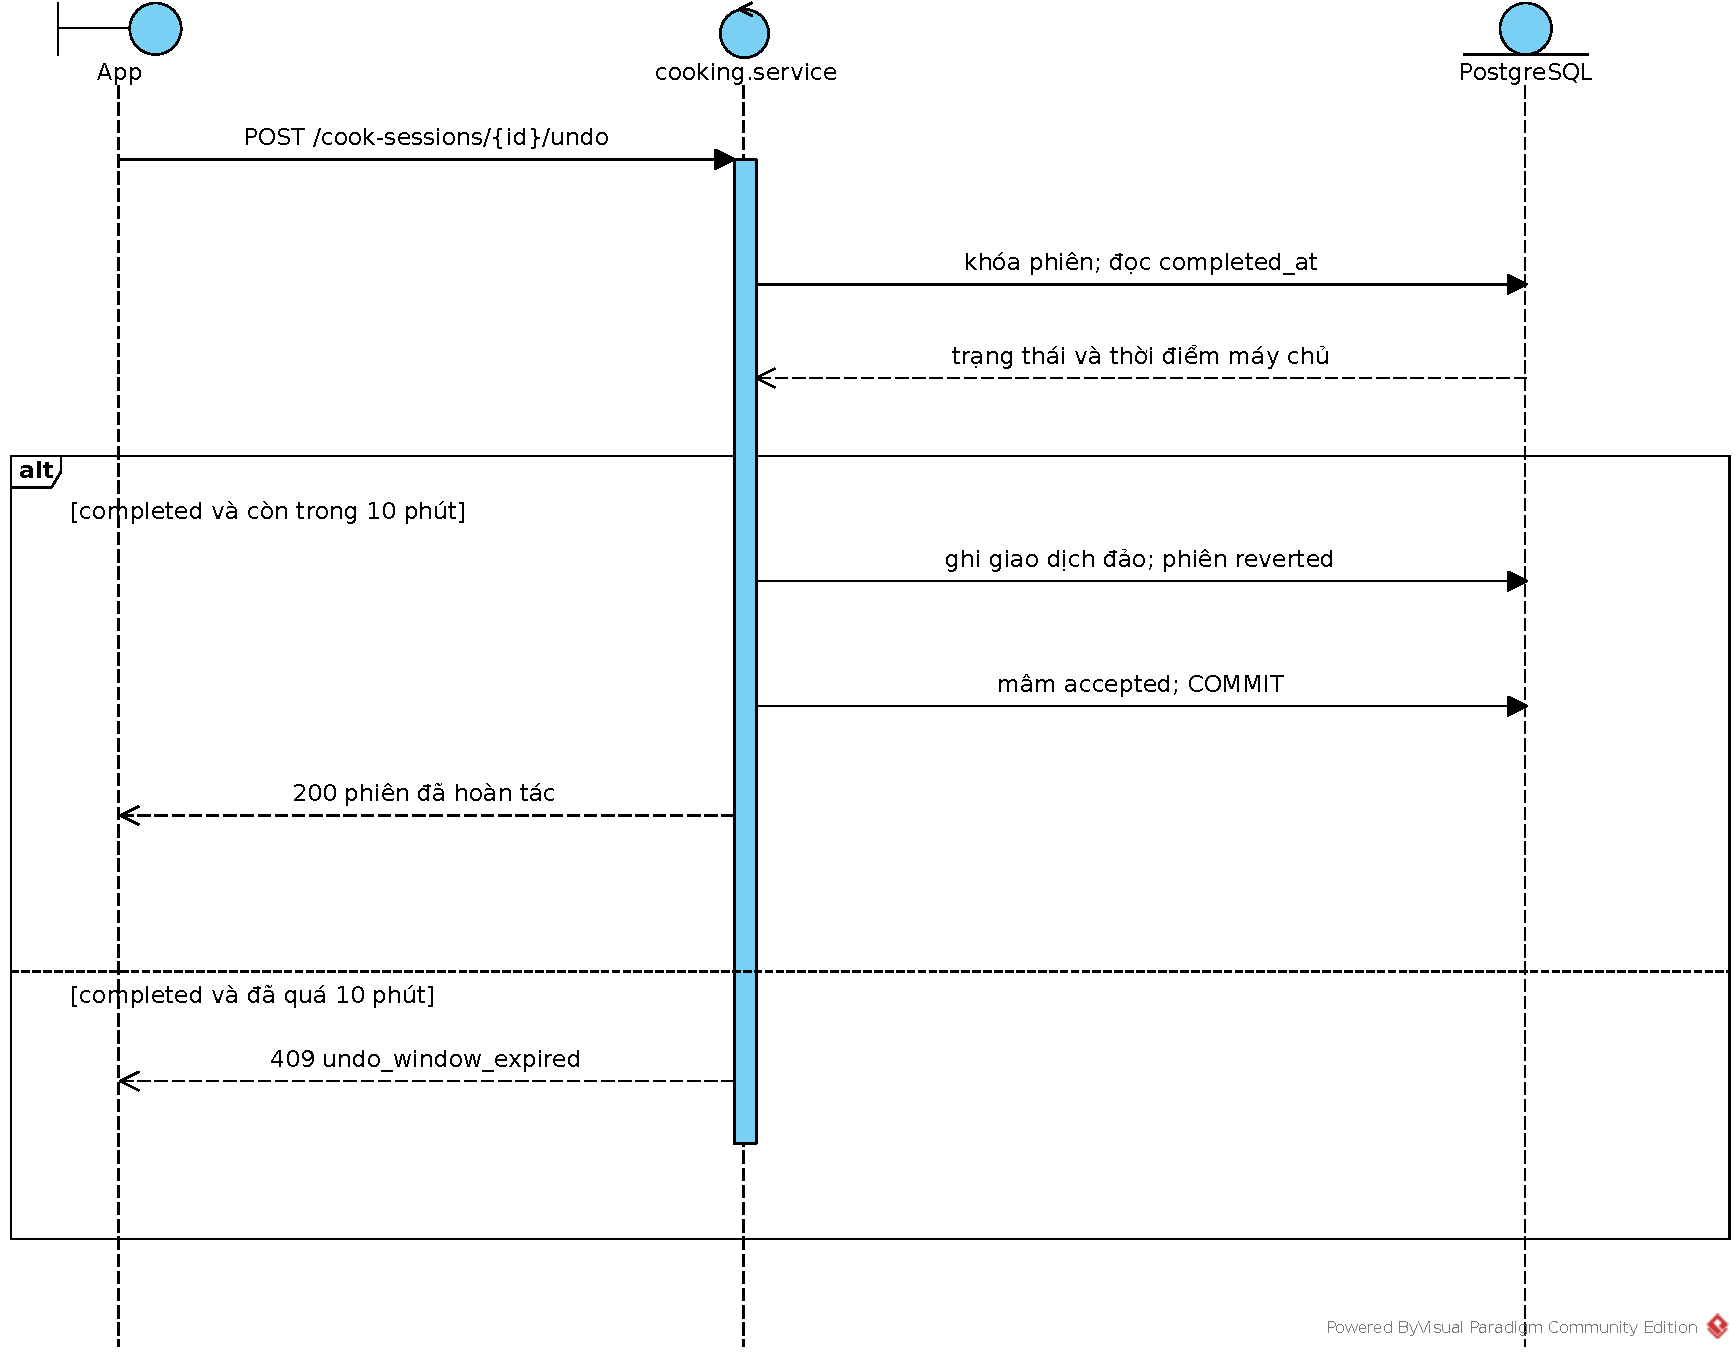
\includegraphics[width=0.96\linewidth,height=0.78\textwidth,keepaspectratio]{assets/SQ02.pdf}
\caption{SQ02 --- Hai nhánh thời hạn của hoàn tác; các trạng thái khác xem UC21}\label{fig:Bao-cao-Tastoria:19}
\end{figure}
\end{landscape}\clearpage
Ở mã hiện tại, nếu phiên đã {\small\texttt{completed}}, service trả tóm tắt đã có thay vì trừ kho lần nữa. Điều này khác một số sequence cũ mô tả trả 409 cho mọi phiên không {\small\texttt{in\_\allowbreak{}\allowbreak{}progress}}. Nhánh cùng Idempotency-\allowbreak{}Key được xử lý sớm tại router. Cả hai lớp bảo vệ đều cần test, không chỉ test nút bị vô hiệu hóa trên giao diện.

{\footnotesize\setlength{\tabcolsep}{0pt}
\begin{longtable}{@{}L{5.133cm}@{\hspace{3mm}}L{5.133cm}@{\hspace{3mm}}L{5.133cm}@{}}
\caption{Lịch nấu, hoàn tất, hoàn tác và nhật ký}\\
\toprule
\textbf{Trạng thái phiên trước thao tác} & \textbf{Thao tác /\allowbreak{} điều kiện} & \textbf{Kết quả} \\
\midrule\endfirsthead
\multicolumn{3}{l}{\small\itshape Bảng \thetable{} (tiếp theo)}\\
\toprule
\textbf{Trạng thái phiên trước thao tác} & \textbf{Thao tác /\allowbreak{} điều kiện} & \textbf{Kết quả} \\
\midrule\endhead
\bottomrule\endfoot
in\_\allowbreak{}progress & Hoàn tất hợp lệ & completed; ghi biến động kho và thời điểm máy chủ \\ \addlinespace[3pt]
completed & Gửi lại hoàn tất & Trả tóm tắt hiện có; không trừ lần hai \\ \addlinespace[3pt]
completed & Hoàn tác trong hạn & reverted; ghi đảo; mâm trở lại accepted \\ \addlinespace[3pt]
completed & Hoàn tác quá hạn & Lỗi undo\_\allowbreak{}window\_\allowbreak{}expired; dữ liệu giữ nguyên \\ \addlinespace[3pt]
reverted & Gửi lại hoàn tác & Trả trạng thái đã có; không đảo lần hai \\ \addlinespace[3pt]
in\_\allowbreak{}progress & Bỏ phiên & abandoned; không trừ kho \\ \addlinespace[3pt]
\end{longtable}}
Thời điểm thiết bị báo nấu xong có thể được dùng cho sự kiện sau kiểm tra, nhưng hạn hoàn tác căn cứ completed\_\allowbreak{}at do máy chủ ghi. Hai mốc có vai trò khác nhau; dùng giờ thiết bị cho hạn sẽ làm kết quả phụ thuộc đồng hồ hoặc thời gian gửi lại.

Có hai lớp chống lặp: khóa Idempotency-\allowbreak{}Key trả phản hồi cho cùng yêu cầu; trạng thái completed bảo vệ khi người dùng gửi lại mục tiêu với khóa mới. Khóa phiên ngăn hai luồng đồng thời cùng thấy in\_\allowbreak{}progress. Toàn bộ thao tác phải cùng transaction để lỗi sau ghi kho nhưng trước cập nhật mâm không tạo trạng thái lệch.

Lượng kho thực tế có thể thay đổi từ lúc đề xuất tới lúc hoàn tất. Service trả danh sách shortfalls nếu có thiếu hụt; báo cáo không giả định lời giải hợp lệ lúc tạo mâm bảo đảm tồn kho bất biến mãi về sau. Nhật ký và kết quả hoàn tất cần phản ánh dữ liệu đã ghi thay vì tự suy ra từ thao tác bấm nút.

\subsection{Dữ liệu, mô hình và vận hành}
Danh mục nhập từ nguồn có cấu trúc; mô hình có phiên bản và mã băm; worker nạp artifact đã được chọn. Dữ liệu huấn luyện phải theo phạm vi đồng ý, không lấy mọi ảnh người dùng chỉ vì chúng tồn tại trên máy chủ. Sao lưu và xóa ảnh theo lịch là tác vụ riêng, cần bằng chứng chạy/\allowbreak{}khôi phục.

Frontend CI kiểm TypeScript, lint, export, browser và nginx trước khi promote; máy chủ triển khai web rồi build APK ký. Pipeline này không đồng nghĩa backend/\allowbreak{}model cũng tự động được nghiệm thu và phát hành. Phần khó là đồng bộ model--ánh xạ lớp--tiền xử lý--artifact và giữ khả năng quay lui.

{\footnotesize\setlength{\tabcolsep}{0pt}
\begin{longtable}{@{}L{3.775cm}@{\hspace{3mm}}L{3.775cm}@{\hspace{3mm}}L{3.775cm}@{\hspace{3mm}}L{3.775cm}@{}}
\caption{Dữ liệu, mô hình và vận hành}\\
\toprule
\textbf{Công đoạn} & \textbf{Đầu vào} & \textbf{Kiểm soát cần có} & \textbf{Bằng chứng nghiệm thu} \\
\midrule\endfirsthead
\multicolumn{4}{l}{\small\itshape Bảng \thetable{} (tiếp theo)}\\
\toprule
\textbf{Công đoạn} & \textbf{Đầu vào} & \textbf{Kiểm soát cần có} & \textbf{Bằng chứng nghiệm thu} \\
\midrule\endhead
\bottomrule\endfoot
Biên soạn & Công thức, nguyên liệu, nguồn & Mã danh mục, đơn vị, cấu trúc và nguồn gốc & Log kiểm/\allowbreak{}import đúng phiên bản \\ \addlinespace[3pt]
Khảo sát & Form, món chấm, người tham gia & Phiên bản form và phạm vi đồng ý & Bản xuất có mô tả cấu trúc \\ \addlinespace[3pt]
Đăng ký mô hình & Artifact và metadata & Mã băm, ánh xạ lớp, tiền xử lý & Manifest và báo cáo đánh giá \\ \addlinespace[3pt]
Triển khai/\allowbreak{}quay lui & Phiên bản được chọn & Tương thích worker, khả năng tải artifact & Log chọn phiên bản và yêu cầu kiểm tra \\ \addlinespace[3pt]
Bảo trì & Lịch xóa/\allowbreak{}sao lưu/\allowbreak{}dọn & Phạm vi xóa, quyền tệp, khả năng khôi phục & Log chạy và biên bản restore \\ \addlinespace[3pt]
\end{longtable}}
Các loại bằng chứng trong bảng là điều kiện cần thu thập, không phải tuyên bố đã có đủ. Khả năng mở một endpoint hoặc chạy CLI không chứng minh chất lượng mô hình, cũng không thay thế kiểm thử khôi phục dữ liệu.

\section{Giao dịch, bất đồng bộ và hiệu năng}
Có hai ranh giới cần phân biệt. Ranh giới module giúp phân công và kiểm soát phụ thuộc. Ranh giới transaction bảo đảm một thay đổi nghiệp vụ hoặc được ghi đầy đủ hoặc không ghi. UC13 và UC20 đi qua nhiều module nhưng vẫn dùng cùng session/\allowbreak{}giao dịch; tách chúng thành nhiều HTTP service ngay sẽ làm mất tính nguyên tử nếu chưa có cơ chế điều phối giao dịch phân tán.

Tác vụ nhận diện ảnh không nằm trong giao dịch chờ người dùng. API tạo scan và lưu ảnh, commit bản ghi rồi mới enqueue. Worker nhận nhiệm vụ, chạy mô hình và ghi kết quả; người dùng đọc trạng thái rồi xác nhận bằng một yêu cầu mới. Khoảng lỗi giữa commit và enqueue được xử lý bằng dấu enqueued\_\allowbreak{}at và tác vụ quét bù; do đó ``API đã nhận ảnh'' không có nghĩa ``worker đã nhận nhiệm vụ''.

Frontend web và Android dùng cùng API nghiệp vụ nhưng có vòng đời phát hành khác nhau. Trang công khai không yêu cầu phiên đăng nhập; các tài nguyên riêng kiểm quyền tại API. Kiểm tra route trên trình duyệt chỉ là kiểm giao diện, không chứng minh backend chống truy cập chéo. Tương tự, build APK thành công không chứng minh mô hình nhận diện đạt độ chính xác yêu cầu.

Tác vụ ảnh có retry giới hạn; dữ liệu yêu cầu và trạng thái ở DB giúp quan sát lỗi. Bộ giải lịch nấu có giới hạn thời gian và phương án dự phòng. Request nấu xong dùng khóa lũy đẳng và khóa phiên; ghi phản hồi lũy đẳng trong cùng giao dịch với biến động kho, tránh trường hợp kho đã trừ nhưng không có dấu vết chống lặp.

Khi cần mở rộng, ưu tiên đo nút thắt trước: số job chờ, thời gian suy luận, thời gian ghép mâm, truy vấn chậm và dung lượng ảnh. Có thể thêm worker, cache dữ liệu danh mục bất biến và tách lưu tệp mà vẫn giữ backend modular monolith. Chỉ tách service khi có nhu cầu triển khai/\allowbreak{}scale độc lập và kế hoạch nhất quán dữ liệu rõ.

\section{Thiết kế dữ liệu và lưu trữ}
Mô hình dữ liệu cụ thể hóa các thực thể miền bằng bảng, khóa và ràng buộc. Các hình DB biểu diễn UML class \guillemotleft{}table\guillemotright{}; Phụ lục B cung cấp từ điển cấu trúc theo DDL.

\subsection{Các hình thức lưu trữ}
{\footnotesize\setlength{\tabcolsep}{0pt}
\begin{longtable}{@{}L{5.133cm}@{\hspace{3mm}}L{5.133cm}@{\hspace{3mm}}L{5.133cm}@{}}
\caption{Các hình thức lưu trữ}\\
\toprule
\textbf{Nơi lưu} & \textbf{Dữ liệu} & \textbf{Vai trò và giới hạn} \\
\midrule\endfirsthead
\multicolumn{3}{l}{\small\itshape Bảng \thetable{} (tiếp theo)}\\
\toprule
\textbf{Nơi lưu} & \textbf{Dữ liệu} & \textbf{Vai trò và giới hạn} \\
\midrule\endhead
\bottomrule\endfoot
PostgreSQL & Người dùng, đồng ý, hồ sơ, danh mục, scans, lô kho, giao dịch, mâm, phiên nấu, khảo sát, phiên bản mô hình & Nguồn dữ liệu nghiệp vụ chính; có FK, UNIQUE, CHECK, transaction \\ \addlinespace[3pt]
pgvector & Biểu diễn vector theo thiết kế danh mục/\allowbreak{}mô hình & Không thay thế các bảng và quy tắc lọc nghiệp vụ \\ \addlinespace[3pt]
Tệp trên máy chủ & Ảnh quét, artifact mô hình, tệp xuất & DB giữ khóa tham chiếu; nginx chỉ tải sau kiểm quyền ở API \\ \addlinespace[3pt]
Valkey & Hàng đợi RQ, tín hiệu tiến độ và trạng thái tạm & Không coi là sổ kho lâu dài \\ \addlinespace[3pt]
Thiết bị & Cache danh mục/\allowbreak{}lịch nấu, outbox & Dùng khi mất mạng; gửi lại giữ khóa yêu cầu, không quyết định tồn kho cuối cùng \\ \addlinespace[3pt]
Bộ dữ liệu ngoại tuyến & YAML, nguồn dinh dưỡng, dữ liệu huấn luyện & Có phiên bản và nguồn; không nhầm với DB giao dịch đang chạy \\ \addlinespace[3pt]
\end{longtable}}
\subsection{Bảng, khóa và quan hệ}
Các hình dưới chọn cột phục vụ giải thích; từ điển bảng đầy đủ được sinh từ {\small\texttt{db/\allowbreak{}\allowbreak{}schema.\allowbreak{}sql}} trong phụ lục. Kiểu cột/\allowbreak{}PK/\allowbreak{}FK lấy từ DDL, không suy từ tên màn hình. Quan hệ nhiều--nhiều giữa công thức và nguyên liệu được chuyển thành {\small\texttt{recipe\_\allowbreak{}\allowbreak{}ingredients}} có lượng gam.

\begin{figure}[H]\centering
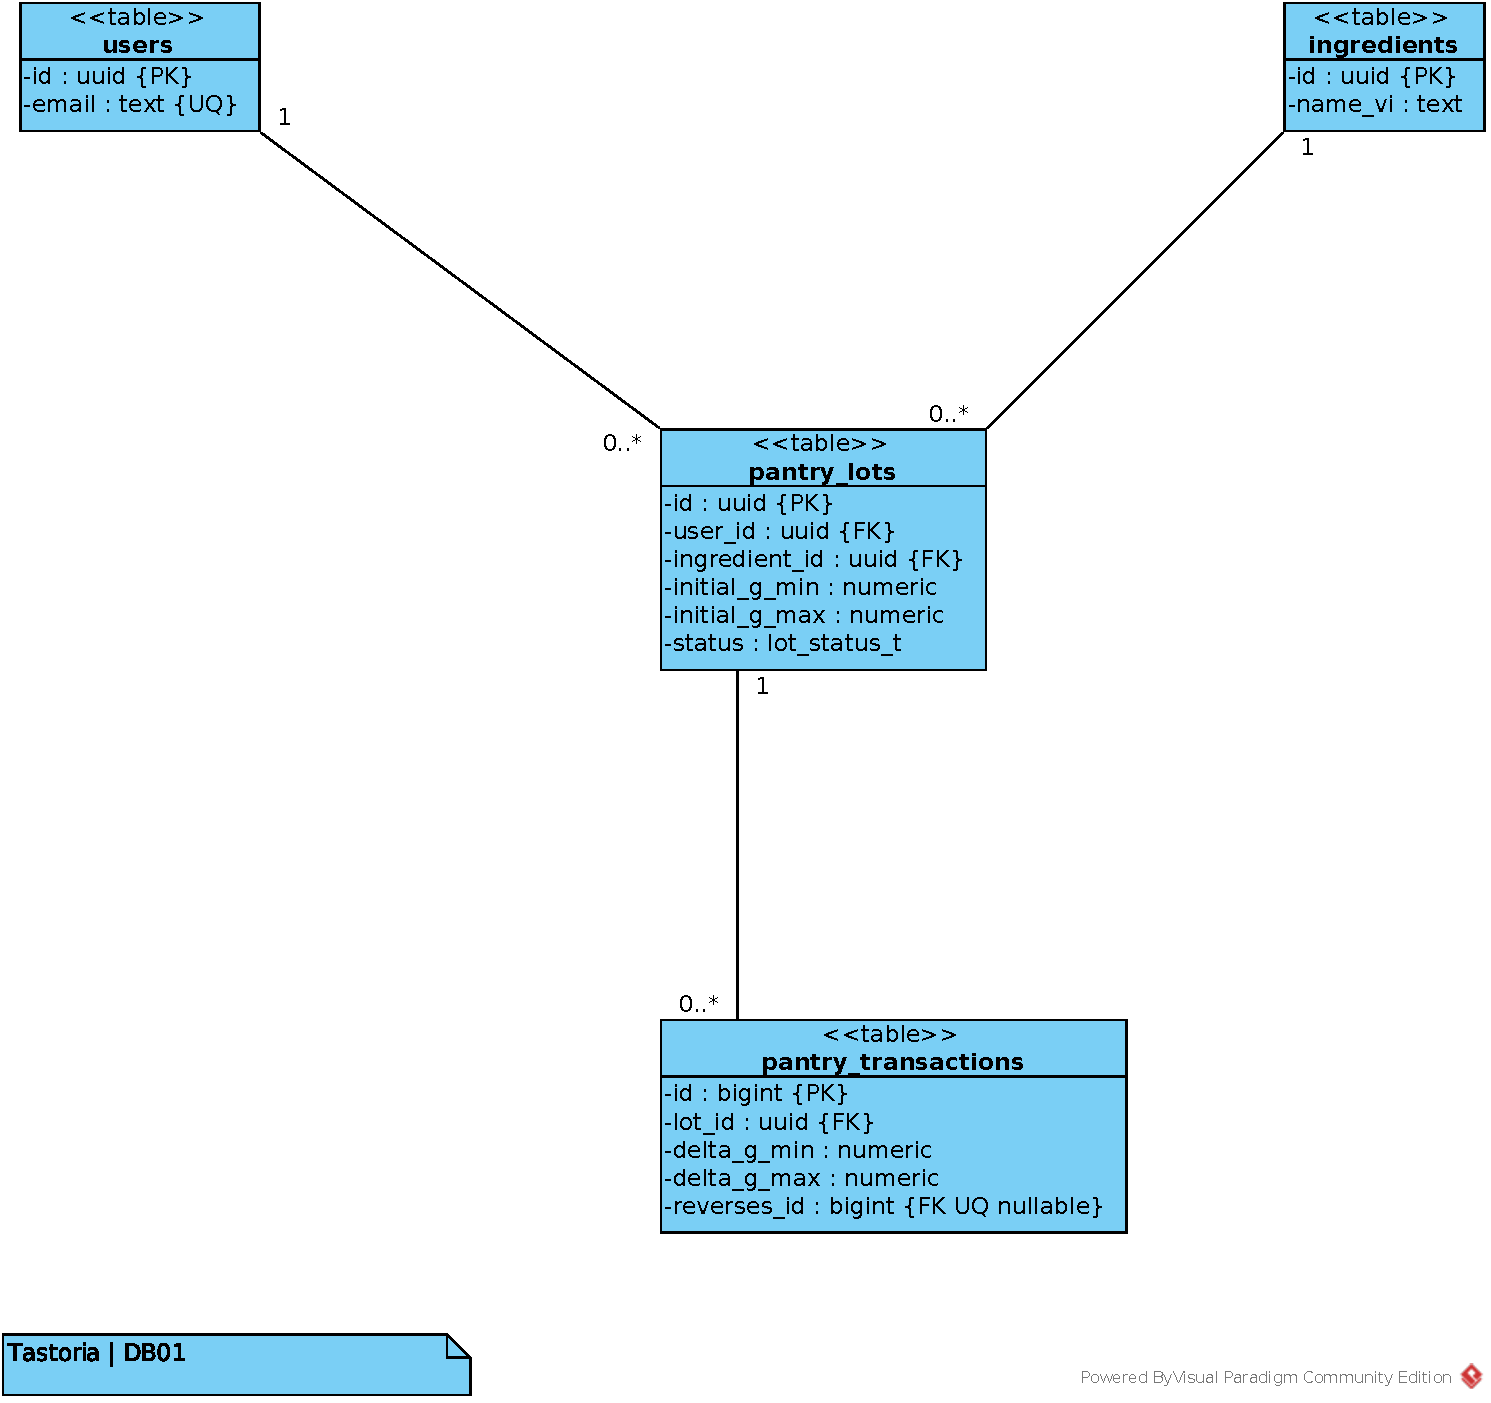
\includegraphics[width=0.96\linewidth,height=0.75\textheight,keepaspectratio]{assets/DB01.pdf}
\caption{DB01 --- Cấu trúc kho và lịch sử}\label{fig:Bao-cao-Tastoria:20}
\end{figure}
{\small\texttt{pantry\_\allowbreak{}\allowbreak{}transactions.\allowbreak{}lot\_\allowbreak{}\allowbreak{}id}} bắt buộc tham chiếu một lô. {\small\texttt{reverses\_\allowbreak{}\allowbreak{}id}} là FK tự tham chiếu nullable và UNIQUE: một giao dịch trừ có tối đa một bản ghi đảo. Hình DB01 giản lược cạnh tự tham chiếu để dễ đọc; ràng buộc vẫn được liệt kê trong bảng đầy đủ. {\small\texttt{ref\_\allowbreak{}\allowbreak{}type/\allowbreak{}\allowbreak{}ref\_\allowbreak{}\allowbreak{}id}} là cặp tham chiếu nghiệp vụ đa loại, không được trình bày như một FK thực khi DDL không có FK.

\clearpage\begin{landscape}
\begin{figure}[H]\centering
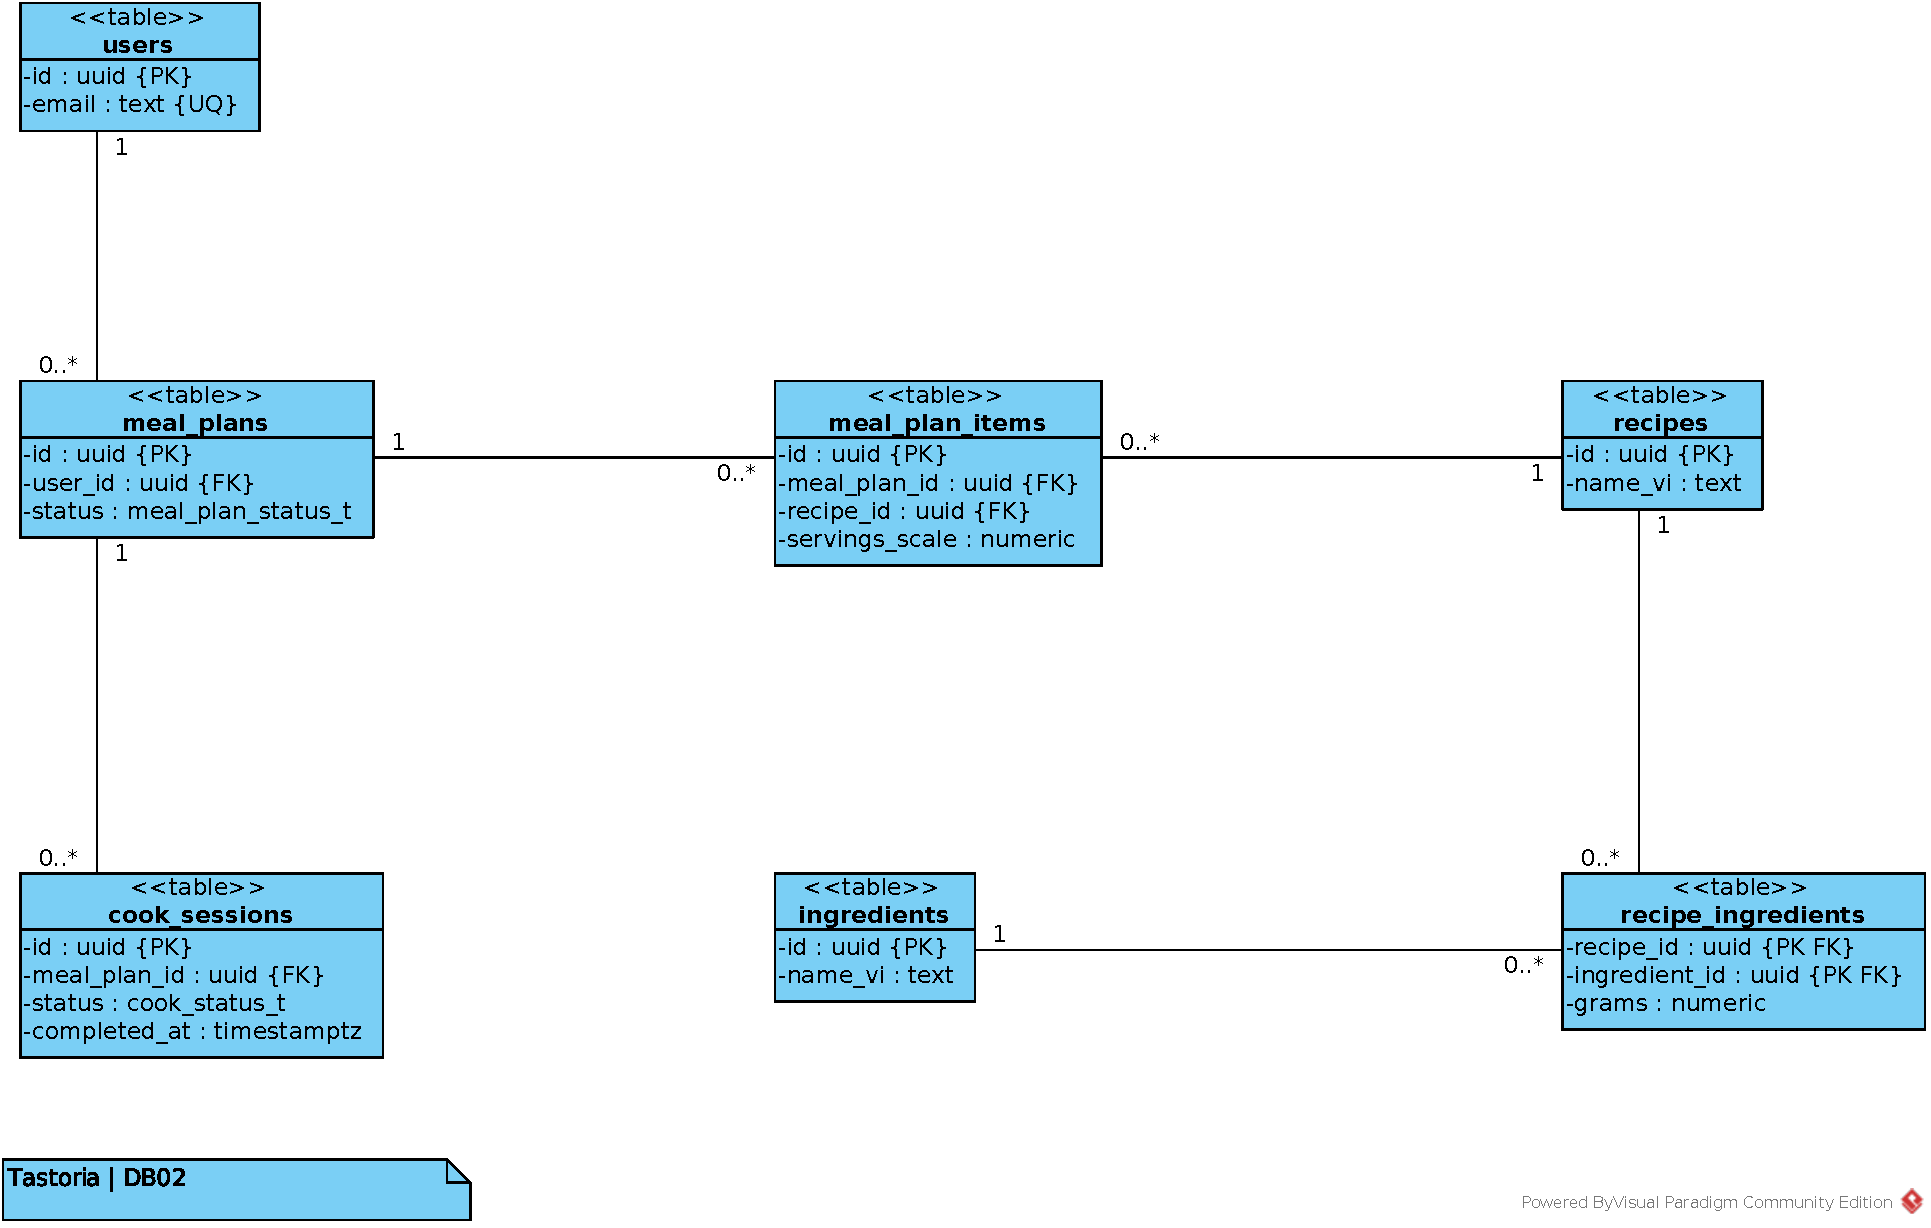
\includegraphics[width=0.96\linewidth,height=0.78\textwidth,keepaspectratio]{assets/DB02.pdf}
\caption{DB02 --- Công thức, mâm và phiên nấu}\label{fig:Bao-cao-Tastoria:21}
\end{figure}
\end{landscape}\clearpage
{\small\texttt{recipe\_\allowbreak{}\allowbreak{}ingredients}} có PK ghép {\small\texttt{(recipe\_\allowbreak{}\allowbreak{}id, ingredient\_\allowbreak{}\allowbreak{}id)}}. {\small\texttt{meal\_\allowbreak{}\allowbreak{}plan\_\allowbreak{}\allowbreak{}items}} giữ lịch sử món thay thế qua {\small\texttt{replaced\_\allowbreak{}\allowbreak{}item\_\allowbreak{}\allowbreak{}id}}; công thức và vị trí món được kiểm bằng FK ghép {\small\texttt{(recipe\_\allowbreak{}\allowbreak{}id, slot)}}. Một mâm có thể có nhiều phiên theo thời gian; ràng buộc một phiên đang nấu cần xem index/\allowbreak{}logic dịch vụ, không thay bội số toàn lịch sử thành 1--1.

\begin{figure}[H]\centering
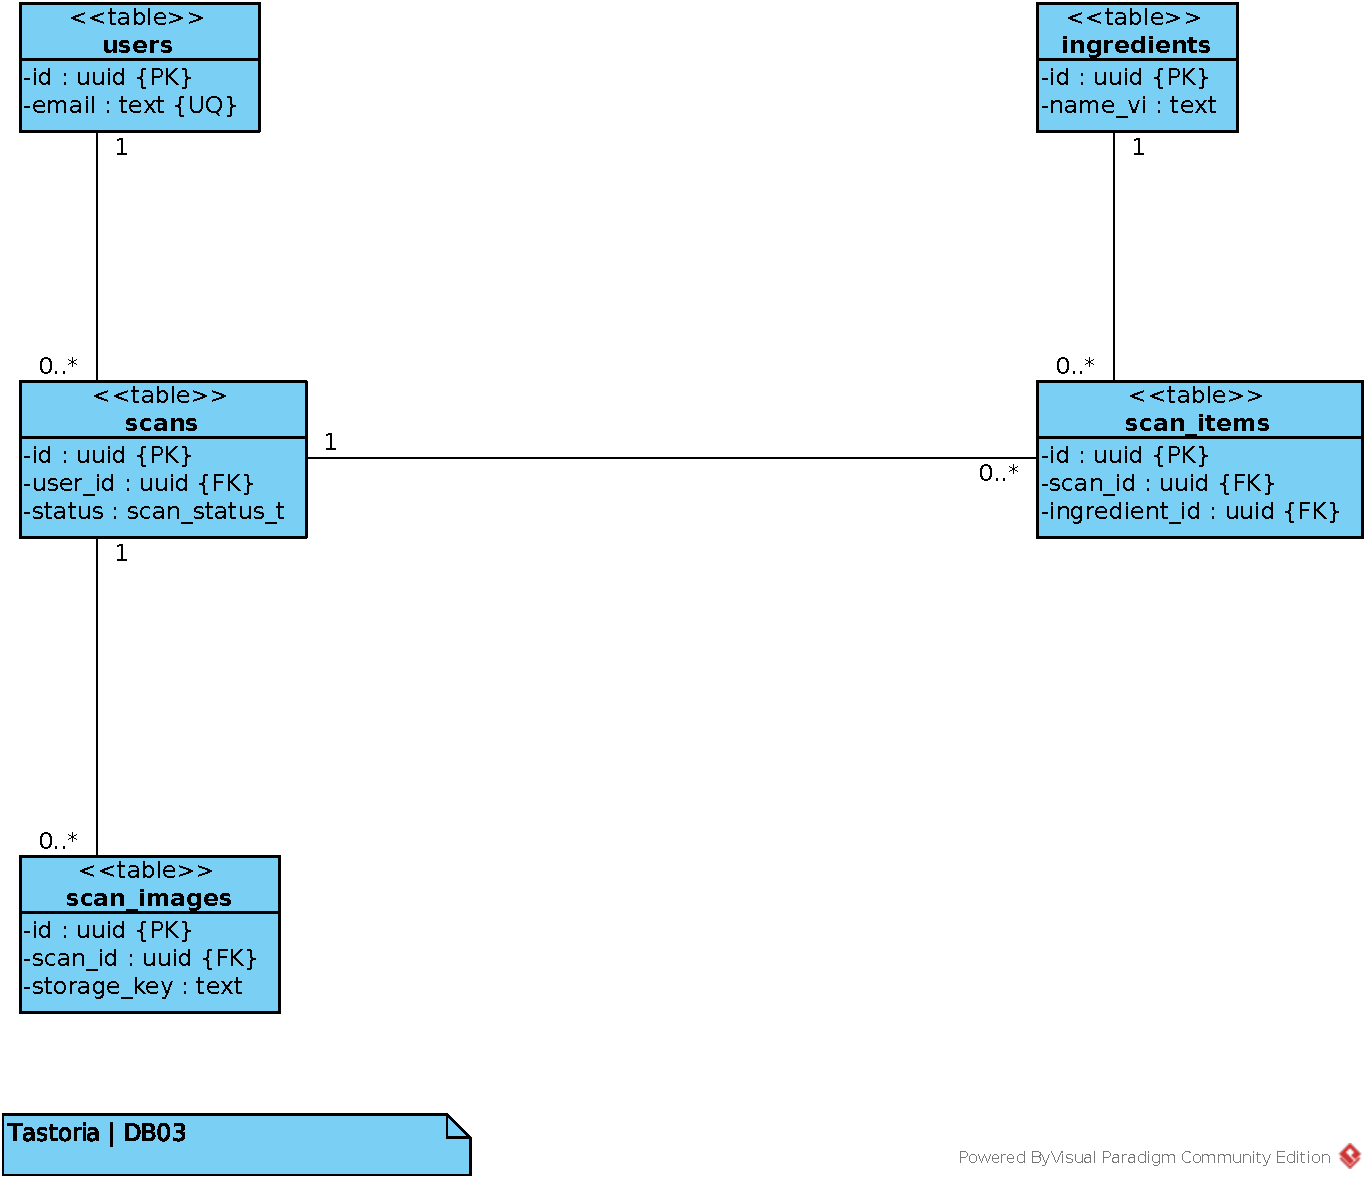
\includegraphics[width=0.96\linewidth,height=0.75\textheight,keepaspectratio]{assets/DB03.pdf}
\caption{DB03 --- Lần quét, ảnh và kết quả}\label{fig:Bao-cao-Tastoria:22}
\end{figure}
Mỗi ảnh/\allowbreak{}kết quả thuộc một lần quét. Scan thuộc đúng một người dùng. Ảnh thô và lô kho không đồng nhất: phải qua bước xác nhận rồi mới phát sinh thay đổi kho. {\small\texttt{detections}} lưu khung phát hiện; {\small\texttt{scan\_\allowbreak{}\allowbreak{}items}} là kết quả nghiệp vụ đã gộp/\allowbreak{}sửa.

\subsection{Chuẩn hóa và dữ liệu dẫn xuất}
Tách người dùng, nguyên liệu, công thức và lô kho để tránh lặp dữ liệu danh mục trong giao dịch. Các quan hệ nhiều--nhiều có bảng nối, không lưu danh sách mã bằng chuỗi phân cách. Đơn vị/\allowbreak{}nhóm dị ứng là danh mục, không rải nhãn tự do trong nhiều bảng.

Số dư kho là giá trị tính từ lượng ban đầu và các giao dịch; mức ưu tiên dùng phụ thuộc thời gian nên cần tính lại khi đọc. Ngược lại, giá trị ảnh chụp tại lúc lập mâm hoặc hoàn tất nấu được giữ để lịch sử không thay đổi khi danh mục cập nhật. Không kết luận mọi bảng đều đạt BCNF chỉ vì đã có khóa chính; phải xét khóa ứng viên và phụ thuộc hàm từng bảng. Phụ lục cũ về chuẩn hóa là tài liệu tham khảo để nhóm rà soát, không được dùng như chứng nhận tự động.

\subsection{Bất biến giao dịch}
Giả sử lô có khoảng 400--500 g. Sau khi ghi giảm 150 g, còn 250--350 g. Gửi lại cùng thao tác không ghi thêm dòng giảm. Khi hoàn tác hợp lệ, thêm dòng +150 g tham chiếu dòng -150 g; số dư trở lại 400--500 g. Không sửa mất dấu giao dịch cũ. Nếu lỗi trước commit, cả cập nhật phiên và dòng biến động phải rollback.

\section{Thiết kế giao diện theo luồng sử dụng}
Giao diện được trình bày theo chức năng và điểm quyết định của người dùng. Ảnh chụp hiện có minh họa bố cục, không thay thế kiểm thử trạng thái lỗi, quyền truy cập hoặc hiệu năng.

\subsection{Tài khoản, hồ sơ và quyền dữ liệu}
\begin{figure}[H]\centering
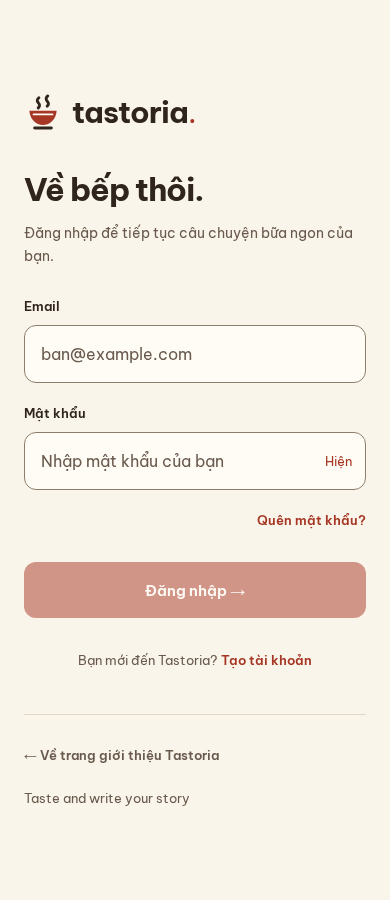
\includegraphics[width=0.85\linewidth,height=0.75\textheight,keepaspectratio]{assets/ui-dang-nhap-2026-10-30.png}
\caption{Màn đăng nhập đã cập nhật, ảnh chụp ngày 30/\allowbreak{}10/\allowbreak{}2026}\label{fig:Bao-cao-Tastoria:23}
\end{figure}
Form có email, mật khẩu, hiện/\allowbreak{}ẩn mật khẩu, khôi phục và chuyển đăng ký. Trên desktop form đi cùng ảnh chụp thật; mobile ưu tiên form. Landing vẫn truy cập công khai. Ảnh này là bằng chứng bố cục, không phải bằng chứng đã kiểm thử mọi lỗi bảo mật.

\subsection{Quét ảnh và quản lý kho theo lô}
\begin{figure}[H]\centering
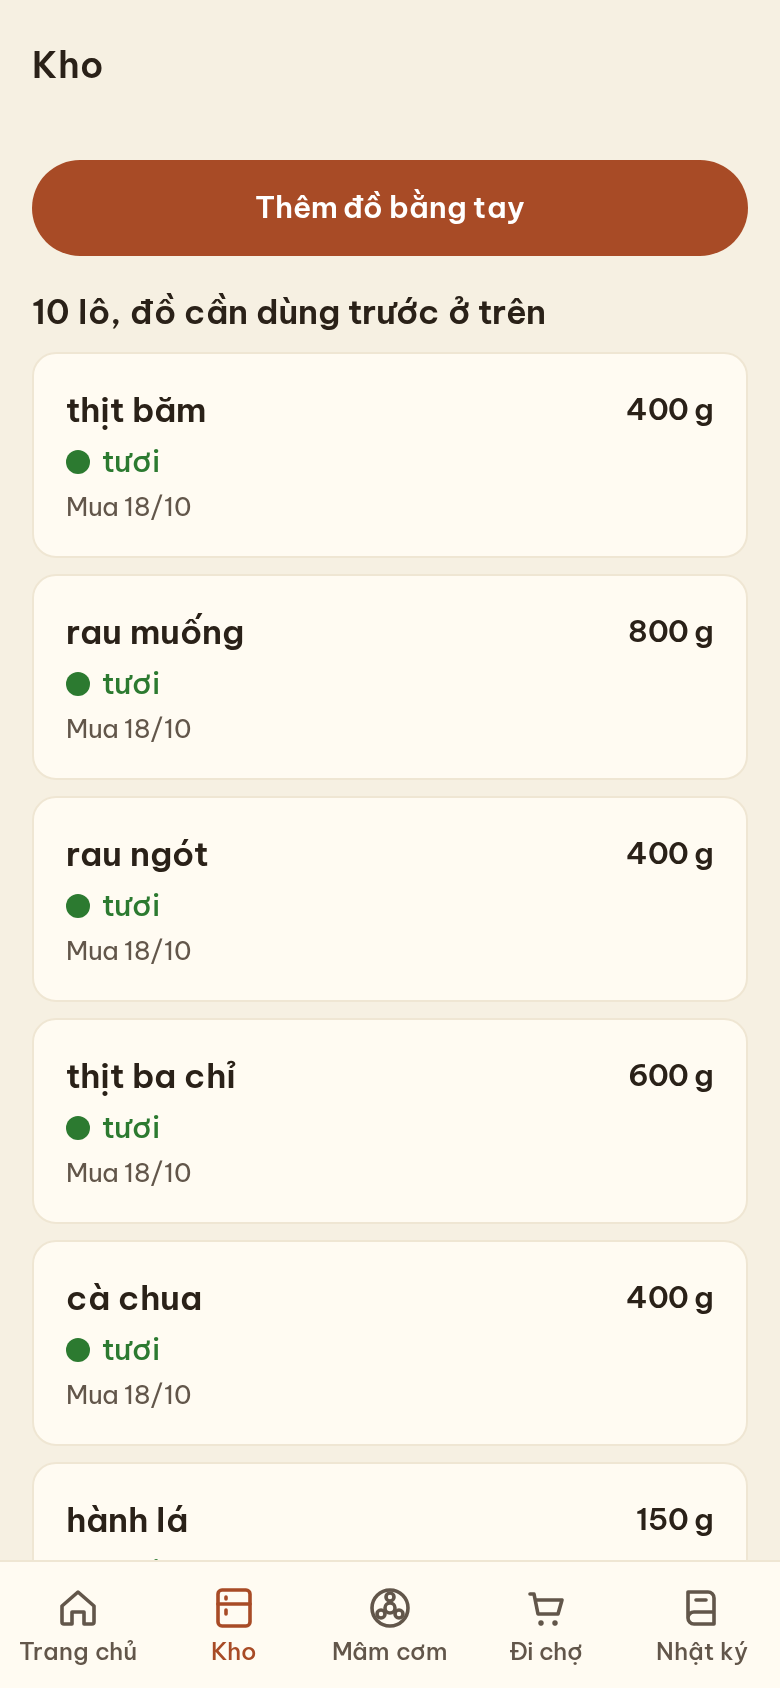
\includegraphics[width=0.85\linewidth,height=0.75\textheight,keepaspectratio]{assets/ui-12-kho-light.png}
\caption{Kho nguyên liệu theo lô --- ảnh minh họa từ bộ kiểm thử giao diện của dự án}\label{fig:Bao-cao-Tastoria:24}
\end{figure}
Màn quét cần hiển thị trạng thái rõ; màn xác nhận cho sửa tên, số lượng, nguồn lô. Màn kho hiển thị lượng/\allowbreak{}ngày nhập/\allowbreak{}ưu tiên sử dụng bằng chữ, không chỉ chấm màu. Ảnh nghiệp vụ trong mục 2 lấy từ bộ ảnh kiểm thử có sẵn, không phải dữ liệu người dùng thật.

\subsection{Gợi ý mâm, đổi món và đi chợ}
\begin{figure}[H]\centering
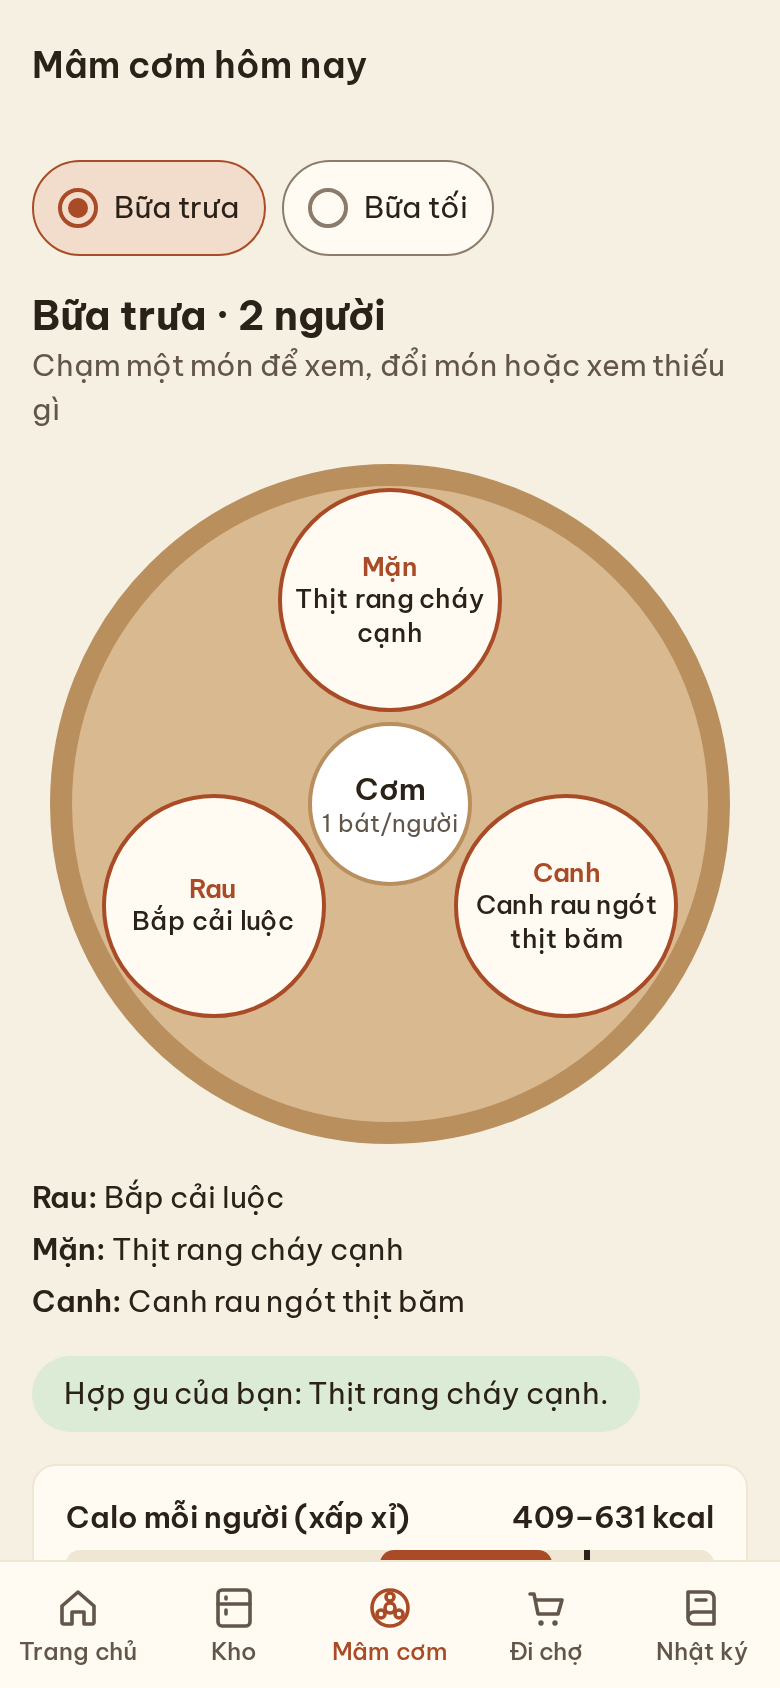
\includegraphics[width=0.85\linewidth,height=0.75\textheight,keepaspectratio]{assets/ui-14-mam-com-hom-nay-light.png}
\caption{Mâm cơm hôm nay --- ảnh từ bộ kiểm thử giao diện}\label{fig:Bao-cao-Tastoria:25}
\end{figure}
Thẻ món cần có vị trí, lượng/\allowbreak{}khẩu phần, lý do gợi ý và đường đi tới đổi món hoặc nguyên liệu thiếu. Khi không còn ứng viên thay thế, giữ mâm hiện tại và giải thích, không hiện nút có vẻ thao tác được nhưng không có kết quả.

\subsection{Lịch nấu, hoàn tất, hoàn tác và nhật ký}
\begin{figure}[H]\centering
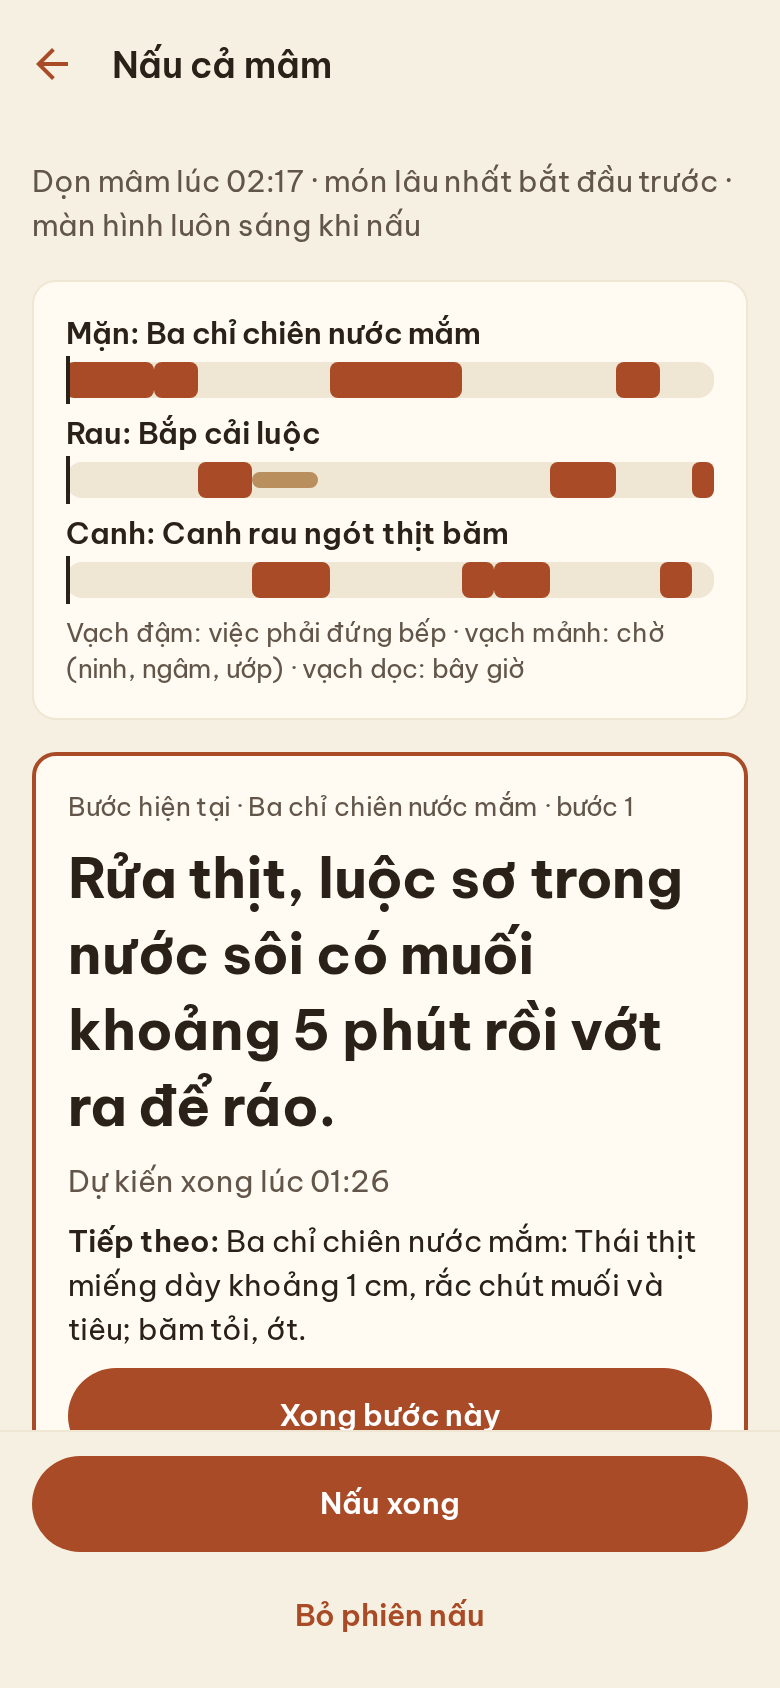
\includegraphics[width=0.85\linewidth,height=0.75\textheight,keepaspectratio]{assets/ui-20-nau-ca-mam-light.png}
\caption{Nấu cả mâm --- ảnh từ bộ kiểm thử giao diện}\label{fig:Bao-cao-Tastoria:26}
\end{figure}
Lịch cần thể hiện các bước có thể chờ và bước cần thao tác. Màn hoàn tất hiển thị đã trừ những lô nào và thời hạn hoàn tác. Nếu outbox đang chờ, trạng thái phải khác với ``máy chủ đã xác nhận''.

\subsection{Dữ liệu, mô hình và vận hành}
Khảo sát có màn hình chọn/\allowbreak{}chấm món trong app/\allowbreak{}web. Các công việc vận hành dùng CLI/\allowbreak{}API và công cụ gán nhãn; không vẽ một trang quản trị chưa được xây dựng rồi gọi là ``giao diện đã hoàn thành''. Khi nghiệm thu vận hành, cần bổ sung ảnh đầu ra CLI hoặc công cụ thật, che bí mật và ghi môi trường chạy.
